\thispagestyle{headfootimage}

Os objetivos e metas deste produto estão alinhados com a \gls{pnrs}, \gls{pnsb}, as normas das três esferas de poder e também com os \gls{ods}.

O prognóstico do sistema de manejo de resíduos sólidos foi projetado para o horizonte de 20 anos de vigência do plano (período de 2019 a 2039) As estimativas da geração de resíduos por classe foram baseadas nas taxas de geração do diagnóstico (Produto 3) e na projeção da população no período. É importante ressaltar que ...

\subsection{Metas}
Criação de um grupo de apoio mútuo para comprimento das metas e objetivos estabelecidos neste plano. O grupo deverá contar com representantes do poder público, da sociedade civil e pessoal técnico e capacitado. Parceria com instituições para apoio técnico.

Reativação do Conselho Municipal de Meio Ambiente para implementação do plano e afins.


\newpage
\FloatBarrier
\section{Identificação de áreas favoráveis para disposição final ambientalmente adequada}
\label{sec:areas_fav}
%% manual item II
%% Entrega X: XX.nov.2019
%% autora: indefinido, verificar possibilidade com a MYR

\newpage
\FloatBarrier
\section{Identificação das possibilidades de soluções consorciadas ou compartilhadas com outros municípios}
\label{sec:sol_cons}

%% Manual item III
%% Entrega 1: 30.nov.2019
%% Autora: Laís Shiki


A \gls{pnrs} estabelece que os municípios que optarem por soluções consorciadas intermunicipais para a gestão dos resíduos sólidos, seguindo as diretrizes da Lei Federal n° 11.107/2005 que regulamenta os consórcios públicos, terão prioridade no acesso aos recursos da União \cite{brasil:12305}. Porém, é necessário cautela na escolha dos municípios a serem estabelecidos tais contratos. Segundo o Manual de Referência para elaboração do \gls{pmgirs} da \gls{agevap}, deve-se considerar a proximidade entre os locais, a possibilidade de compartilhamento de pessoal técnico, equipamentos e infraestrutura e as formas de prevenção de riscos ambientais com a perspectiva de economia de escala \cite{agevap_manual_2019}.

\subsection{Etapas para criação de um consórcio público}

Segundo a \gls{cnm}, as seguintes etapas devem ser seguidas a fim de se estabelecer um consórcio público intermunicipal \cite{consorcio_publico}: 

\begin{itemize}
	\item \textbf{Identificar os interesses e problemas em comum -} para se realizar o levantamento das dificuldades e problemas, é recomendável que sejam feitas reuniões/audiências públicas contendo a presença de agentes públicos de ambos municípios, a sociedade civil e uma equipe de trabalho técnica multidisciplinar;   
	
	\item \textbf{Elaborar Estudos de Viabilidade -} a equipe técnica deverá levantar as maneiras adequadas para resolver as necessidades identificadas, os passos a serem seguidos, os prazos e custos para desenvolver tal solução consorciada;
	
	\item \textbf{Elaborar o Protocolo de Intenções -} de acordo com o Art. 4° da Lei Federal n° 11.107/2005, o Protocolo de Intenções deve conter:
	\subitem I – a denominação, as finalidades, o prazo de duração e a
	sede do consórcio público, admitindo-se a fixação de prazo
	indeterminado e a previsão de alteração da sede mediante
	decisão da Assembleia-Geral;
	\subitem II – a identificação de cada um dos Entes da Federação
	que podem vir a integrar o consórcio público, podendo indicar prazo para que subscrevam o protocolo de intenções;
	\subitem III – a indicação da área de atuação do consórcio público;
	\subitem IV – a previsão de que o consórcio público é associação
	pública, com personalidade jurídica de direito público e
	natureza autárquica, ou pessoa jurídica de direito privado;
	\subitem V – os critérios para, em assuntos de interesse comum, autorizar o consórcio público a representar os Entes da Federação consorciados perante outras esferas de governo;
	\subitem VI – as normas de convocação e funcionamento da assembleia-geral, inclusive para a elaboração, aprovação e modificação dos estatutos do consórcio público;
	\subitem VII – a previsão de que a assembleia-geral é a instância
	máxima do consórcio público e o número de votos para as
	suas deliberações;
	\subitem VIII – a forma de eleição e a duração do mandato do representante legal do consórcio público que, obrigatoriamente,
	deverá ser Chefe do Poder Executivo de Ente da Federação consorciado;
	\subitem IX – o número, as formas de provimento e a remuneração
	dos empregados do consórcio público;
	\subitem X – os casos de contratação por tempo determinado para
	atender à necessidade temporária de excepcional interesse público;
	\subitem XI – as condições para que o consórcio público celebre
	contrato de gestão, nos termos da Lei 9.649, de 1998, ou
	termo de parceria, na forma da Lei 9.790, de 1999;
	\subitem XII – a autorização para a gestão associada de serviço público, explicitando: a) competências cuja execução será transferida ao
	consórcio público;
	b) os serviços públicos objeto da gestão associada
	e a área em que serão prestados;
	c) a autorização para licitar e contratar concessão,
	permissão ou autorizar a prestação dos serviços;
	d) as condições a que deve obedecer ao contrato
	de programa, no caso de nele figurar como contratante o consórcio público; e
	e) os critérios técnicos de cálculo do valor das tarifas e de outros preços públicos, bem como os critérios gerais a serem observados em seu reajuste
	ou revisão.
	\subitem XIII – o direito de qualquer dos contratantes, quando adimplentes com as suas obrigações, de exigir o pleno cumprimento das cláusulas do contrato de consórcio público.
	
	\item \textbf{Ratificar o Protocolo de Intenções -} o passo seguinte é o envio, pelos Poderes Executivos signatários, do Projeto de Lei de ratificação do Protocolo de Intenções para a Câmara Municipal de Vereadores. A ratificação do Protocolo de Intenções é dispensada quando o Ente da Federação que, antes de subscrever o Protocolo de Intenções, disciplinar por lei a sua participação no consórcio público, de forma a poder assumir todas as obrigações previstas no referido	documento. Por conta da agilidade e desburocratização, diversos municípios têm procedido dessa forma, utilizando o que se convenciona chamar “Lei Autorizativa” para abreviar a etapa da ratificação;
	
	\item \textbf{Elaborar o Estatuto do Consórcio Público -} o Estatuto, que deve ser aprovado em Assembleia Geral, é o documento que regulamentará a organização e o funcionamento de cada órgão constitutivo do consórcio público e deverá atender todas as cláusulas do Protocolo de Intenções ratificado. Para a sua validação, o Estatuto do Consórcio Público de direito público deverá ser publicado na imprensa oficial no	âmbito de cada Ente consorciado.
\end{itemize}

Uma vez constituído o consórcio público, é importante firmar o Contrato de rateio, que é o meio pelo qual os Entes consorciados comprometem-se a fornecer recursos financeiros para a realização das despesas do consórcio público (Art. 2º, VII, do Decreto 6.017/2007). Mas para isso, em respeito à legislação fiscal, é necessário que cada Ente consorciado faça os devidos ajustes em suas normas orçamentárias \cite{consorcio_publico}.

\subsection{Perspectiva para gestão associada com municípios da região}

Monteiro Lobato é um dos municípios associados ao \gls{codivap}, que visa ser um órgão representativo dos interesses das prefeituras do Vale do Paraíba e litoral norte. Entre esses interesses, destacam-se os referentes ao meio ambiente e recursos hídricos. Portanto, efetuar um consórcio com algum dos municípios integrantes do \gls{codivap} seria de grande interesse a Monteiro Lobato. Na \autoref{tab:municipios_codivap} é apresentado os municípios integrantes, assim como suas respectivas populações e distância deste à Monteiro Lobato.

% Table generated by Excel2LaTeX from sheet 'municipios_codivap'

\begin{table}[htbp]
  \centering
  \arrayrulecolor{white}
 	
  \caption{Municípios integrantes do CODIVAP}
    \resizebox{\textwidth}{!}{%
    \begin{tabular}{c|c|c}
    \rowcolor[rgb]{ .969,  .588,  .275} \textcolor[rgb]{ 1, 1, 1} {Município} & \textcolor[rgb]{ 1, 1, 1} {População estimada (hab) (IBGE, 2019)} & \textcolor[rgb]{ 1, 1, 1} {Distância até Monteiro Lobato (km)} \\
    \rowcolor[rgb]{ .984,  .831,  .706} Aparecida & 36.157 & 85,2 \\
    \rowcolor[rgb]{ .992,  .914,  .851} Arapeí & 2.469  & 212 \\
    \rowcolor[rgb]{ .984,  .831,  .706} Areias & 3.886  & 161 \\
    \rowcolor[rgb]{ .992,  .914,  .851} Bananal & 10.945 & 241 \\
    \rowcolor[rgb]{ .984,  .831,  .706} Caçapava & 94.263 & 27,2 \\
    \rowcolor[rgb]{ .992,  .914,  .851} Cachoeira Paulista & 33.327 & 117 \\
    \rowcolor[rgb]{ .984,  .831,  .706} Campos do Jordão & 52.088 & 57,4 \\
    \rowcolor[rgb]{ .992,  .914,  .851} Canas & 5.138  & 110 \\
    \rowcolor[rgb]{ .984,  .831,  .706} Caraguatatuba & 121.532 & 122 \\
    \rowcolor[rgb]{ .992,  .914,  .851} Cruzeiro & 82.238 & 133 \\
    \rowcolor[rgb]{ .984,  .831,  .706} Cunha & 21.547 & 137 \\
    \rowcolor[rgb]{ .992,  .914,  .851} Guararema & 29.798 & 74,9 \\
    \rowcolor[rgb]{ .984,  .831,  .706} Guaratinguetá & 121.798 & 92,2 \\
    \rowcolor[rgb]{ .992,  .914,  .851} Igarata & 9.534  & 78,2 \\
    \rowcolor[rgb]{ .984,  .831,  .706} Ilhabela & 34.970 & 153 \\
    \rowcolor[rgb]{ .992,  .914,  .851} Jacareí & 233.662 & 51,6 \\
    \rowcolor[rgb]{ .984,  .831,  .706} Jambeiro & 6.602  & 70,5 \\
    \rowcolor[rgb]{ .992,  .914,  .851} Lagoinha & 4.896  & 103 \\
    \rowcolor[rgb]{ .984,  .831,  .706} Lavrinhas & 7.260  & 137 \\
    \rowcolor[rgb]{ .992,  .914,  .851} Lorena & 88.706 & 105 \\
    \rowcolor[rgb]{ .984,  .831,  .706} Mogi das Cruzes & 445.842 & 104 \\
    \rowcolor[rgb]{ .992,  .914,  .851} Monteiro Lobato & 4.653  & ------ \\
    \rowcolor[rgb]{ .984,  .831,  .706} Natividade da Serra & 6.661  & 97,8 \\
    \rowcolor[rgb]{ .992,  .914,  .851} Nazaré Paulista & 18.524 & 108 \\
    \rowcolor[rgb]{ .984,  .831,  .706} Paraibuna & 18.222 & 72,9 \\
    \rowcolor[rgb]{ .992,  .914,  .851} Pindamonhangaba & 168.328 & 62,4 \\
    \rowcolor[rgb]{ .984,  .831,  .706} Piquete & 13.657 & 121 \\
    \rowcolor[rgb]{ .992,  .914,  .851} Potim & 24.643 & 87,4 \\
    \rowcolor[rgb]{ .984,  .831,  .706} Queluz & 13.420 & 147 \\
    \rowcolor[rgb]{ .992,  .914,  .851} Redenção da Serra & 3.851  & 75,5 \\
    \rowcolor[rgb]{ .984,  .831,  .706} Roseira & 10.712 & 74,1 \\
    \rowcolor[rgb]{ .992,  .914,  .851} Salesópolis & 17.139 & 94,2 \\
    \rowcolor[rgb]{ .984,  .831,  .706} Santa Branca & \multicolumn{1}{c}{14.788} & 73 \\
    \rowcolor[rgb]{ .992,  .914,  .851} Santa Isabel & 57.386 & 80,5 \\
    \rowcolor[rgb]{ .984,  .831,  .706} Santo Antônio do Pinhal & 6.811  & 36,2 \\
    \rowcolor[rgb]{ .992,  .914,  .851} São Bento do Sapucaí & 10.878 & 42,6 \\
    \rowcolor[rgb]{ .984,  .831,  .706} São José do Barreiro & 4.147  & 183 \\
    \rowcolor[rgb]{ .992,  .914,  .851} São José dos Campos & 721.944 & 39,9 \\
    \rowcolor[rgb]{ .984,  .831,  .706} São Luís do Paraitinga & 10.687 & 84,9 \\
    \rowcolor[rgb]{ .992,  .914,  .851} São Sebastião & 88.980 & 147 \\
    \rowcolor[rgb]{ .984,  .831,  .706} Silveiras & 6.302  & 136 \\
    \rowcolor[rgb]{ .992,  .914,  .851} Taubaté & 314.924 & 46,1 \\
    \rowcolor[rgb]{ .984,  .831,  .706} Tremembé & 47.185 & 64,6 \\
    \rowcolor[rgb]{ .992,  .914,  .851} Ubatuba & 90.799 & 135 \\
    \rowcolor[rgb]{ .984,  .831,  .706} \textbf{TOTAL} & \textbf{3121299} &  \\
    \end{tabular}%
}
  \label{tab:municipios_codivap}%
  \legend{Fonte: Elaborado pelos autores.}
\end{table}%

\FloatBarrier

Com base na \autoref{tab:municipios_codivap}, destacam-se os municípios de Santo Antônio do Pinhal, Caçapava e São José dos Campos, que distam 36,2 km, 27,2 km e 39,9 km, respectivamente. Buscar soluções diretamente com estes municípios, a respeito da gestão de resíduos sólidos, se torna plausível se for considerada a proximidade geográfica entre os locais, que é um dos aspectos relevantes na escolha do município com que será realizado o consórcio.

O município de Monteiro Lobato está estrategicamente localizado no caminho para São Francisco Xavier, distrito de São José dos Campos, sendo assim, uma solução ser o acordo entre os municípios para que o caminhão da coleta seletiva que opera neste distrito também realiza-se a coleta em Monteiro Lobato. Pois, é provável que o caminhão não fique lotado após coleta em São Francisco Xavier.

Outras possibilidades de soluções consorciadas ou compartilhadas que seriam de grande valia para o município são: 
\begin{itemize}
	\item Parcerias com cooperativas de catadores de outros municípios, onde o material coletado em Monteiro Lobato seria enviado para estes locais.Porém, esta medida seria de curto prazo, pois há grande interesse de se implementar uma cooperativa ou outra forma de associação de catadores de materiais recicláveis no próprio município, este assunto será discutido na \autoref{sec:grup_int} e \autoref{sec:mec_renda}.
	
	\item Consórcio com município vizinho para que os rejeitos de Monteiro Lobato sejam encaminhados para o aterro utilizado por este, na hipótese de ocorrer alguma contingência. Por exemplo, Jambeiro possui um aterro sanitário empreendido pelo grupo Engep, que fica em torno de 70 km de distância, o que em casos emergenciais seria uma solução viável.
	
\end{itemize}


\newpage
\FloatBarrier
\section{Identificação dos resíduos sólidos e dos geradores sujeitos ao plano de gerenciamento específico ou ao sistema de logística reversa}
\label{sec:rs_geradores_lr}
% \section{Descrição das formas e dos limites da participação do poder público local na logística reversa} ACHO QUE NÃO É ESSE TÍTULO 
%% Manual item IV
%% Entrega 1: 30.nov.2019
%% Autora: Maysa Rocha

\subsection{Logística reversa}

A Lei 12.305/10 descreve logística reversa como “instrumento de desenvolvimento econômico e social caracterizado por um conjunto de ações, procedimentos e meios destinados a viabilizar a coleta e a restituição dos resíduos sólidos ao setor empresarial, para reaproveitamento, em seu ciclo ou em outros ciclos produtivos, ou outra destinação final ambientalmente adequada”, ou seja, a logística reversa constitui no retorno dos resíduos sólidos para as empresas de origem, o que permite que estes resíduos entrem novamente na cadeia produtiva, diminuindo o consumo de matérias-primas. De acordo com a \gls{pnrs}, a logística reversa passou a vigorar em 2010 e foi regulamentada, devidamente, no ano de 2017, através do Decreto Lei número 9177.

O Art. 33 da \gls{pnrs} define os produtos/resíduos que são obrigados a estruturar e implementar sistemas de logística reversa, mediante retorno dos produtos após uso pelo consumidor, de forma independente do serviço de limpeza urbana e de manejo dos resíduos sólidos. Esses produtos são descritos na Tabela 26, item 1.12 do produto 3: agrotóxicos, seus resíduos e embalagens; pilhas e baterias; pneus; óleo lubrificante, seus resíduos e embalagens; lâmpadas fluorescentes de vapor de sódio e mercúrio e de luz mista; produtos eletroeletrônicos e seus componentes; medicamentos.

O Artigo 20 da PNRS pontua os geradores de resíduos sólidos, que estão definidos no inciso I do art. 13. São eles: 

\begin{itemize}
	\item resíduos dos serviços públicos de saneamento básico: os gerados nessas atividades, 
	\subitem resíduos domiciliares: os originários de atividades domésticas em residências urbanas; 
	\subitem resíduos de limpeza urbana: os originários da varrição, limpeza de logradouros e vias públicas e
	outros serviços de limpeza urbana; 
	\item resíduos industriais: os gerados nos processos produtivos e instalações industriais;  
	\item resíduos de serviços de saúde: os gerados nos serviços de saúde, conforme definido em regulamento ou em normas estabelecidas pelos órgãos do Sisnama e do SNVS; 
	\item resíduos de mineração: os gerados na atividade de pesquisa, extração ou beneficiamento de
	minérios.
\end{itemize}


\subsubsection{Plano de logística reversa - programa de monitoramento}
O grau de responsabilidade do Poder Público é atuante, isto é, não opera o sistema, mas estimula o seu melhor funcionamento, por meio de provimento de recursos para pesquisa e desenvolvimento, financiamento para infraestrutura, campanhas para incentivar o reuso e a coleta dos resíduos, entre outros.

A Decisão de Diretoria da \gls{cetesb} n° 076/2018/C estabeleceu que as empresas sujeitas à implementação de sistemas de logística reversa deverão fornecer à \gls{cetesb} as informações relativas aos seus sistemas por meio do preenchimento de formulários no Módulo Logística Reversa do SIGOR – Sistema Estadual de Gerenciamento Online de Resíduos Sólidos, a ser disponibilizado.

De acordo com a \gls{cetesb}, até o momento os sistemas de LR têm assumido três formatos distintos, definidos em função da forma como os resíduos pós-consumo são coletados. Esses modelos não são obrigatórios, e é desejável que novos arranjos sejam propostos com a experiência das empresas nesse tipo de atividade. Porém, ao menos para o momento, estes três modelos tem se mostrado os mais adequados, podendo inspirar a formatação dos sistemas pelas empresas. Esses modelos são: PEV, coleta seletiva ou central de triagem/entidades de catadores. 

\paragraph{\textbf{Adicionar uma rota de coleta à rota de entrega}}
Os caminhões que vão destinar o resíduo corretamente, quando termina a sua rota de entrega necessita voltar para o depósito. Esse caminho de retorno pode contemplar o recolhimento por exemplo de pneus descartados. O fabricante de pneus e sua transportadora aproveitam melhor a rotina de entregas e otimizam a logística reversa.


\paragraph{\textbf{Parceria com ONGs}}
Parceria entre os fabricantes de pneus, por exemplo e ONG’s, com o intuito de fazer uma horta comunitária. O custo de recolher e encaminhar pneus seria reduzido e com essa economia, o produtor pode incentivar a ONG com a doação de um pequeno utilitário para fazer a coleta. A empresa ganha incentivo fiscal com a doação, a ONG ganha com o veículo. Dessa forma, o município pode colaborar com o incentivo fiscal para empresas retornarem o resíduo a um local que o reutilize.

\paragraph{\textbf{\gls{pev}}}
A URBAM - Urbanizadora Municipal de São José dos Campos define PEV como pontos de entrega voluntária que representam uma área pública instalada em local adequado, cuidadosamente escolhido para receber resíduos. O PEV recebe sobras de obras de construção, reforma ou demolição, (tábuas, tijolos, telhas, fiações, tubulações, pisos e materiais de acabamento) até 1m³ (ou seja, o volume de um porta-malas de carro de passeio ou caçamba de um utilitário), móveis e equipamentos domésticos (sofás, cadeiras, geladeiras, armários), pilhas, bateria; lâmpadas fluorescentes inteiras - até 4 unidades por entrega, sobras de podas de jardim - até 1m³ por entrega, madeira - até 1m³ por entrega, pneus - até 4 por entrega e óleo de cozinha usado. Os PEV’s não recebem lixo orgânico, animais mortos, materiais recicláveis, lixo hospitalar e volumes acima de 1m³.

\paragraph{\textbf{Molécoola}}
Molécoola é uma Startup de impacto, que já coletou mais de 300 toneladas de materiais recicláveis e 100 \% deles foram corretamente destinados. A dinâmica funciona da seguinte forma: 
\begin{itemize}
	\item (1) Baixar o aplicativo no seu celular, cadastrar-se e juntar os recicláveis - é importante que os resíduos recicláveis possuam um tratamento antes de serem levados a esse ponto de coleta, é imprescindível a pré lavagem das embalagens;
	\item (2) Buscar a loja da Molécoola mais próxima no seu celular e levar os recicláveis limpos e separados; 
	\item (3) Cada tipo de material gera uma pontuação diferentes, os materiais serão pesados no local e sincronizados com a sua conta do aplicativo;
	\item (4) Por fim, a sua pontuação gera trocas por produtos, serviços e descontos.
\end{itemize}


\begin{figure}
	\centering
	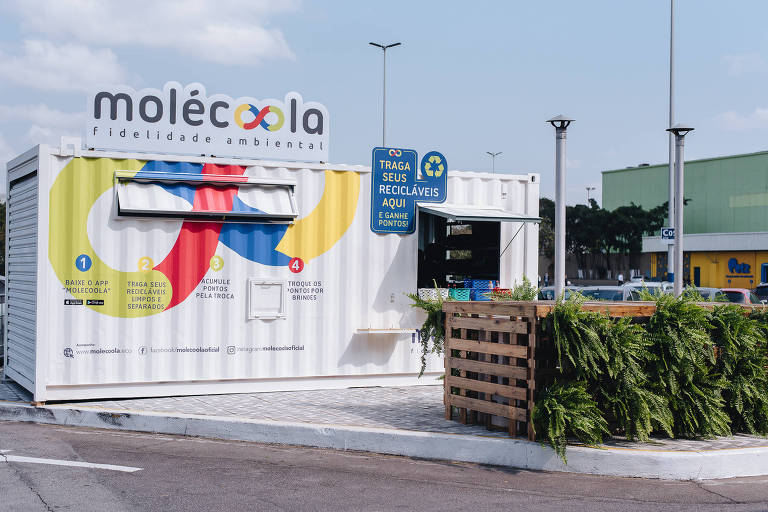
\includegraphics[width=0.7\linewidth]{produtos/prodquatro/molecoola}
	\caption{Contêiner do Molécoola}
	\label{fig:molecoola}
	\legend{Fonte: Jornal Folha de São Paulo}
\end{figure}
\FloatBarrier

\paragraph{\textbf{Armário Coletivo}}
Carina Zagonel é idealizadora do projeto “Armário Coletivo”, que consiste num “movimento de intervenção urbana que utiliza armários para transformar espaços públicos e criar novos hábitos de consumo. Eles são construídos a partir de materiais coletados nas ruas, produzidos com a ajuda da própria comunidade ”. O armário fica em um ponto escolhido estrategicamente no município ou no bairro em questão, os moradores podem ir até os armários e depositarem roupas, objetos que não utilizam mais. O outro morador que passa pelo local, pode abrir o armário e escolher o que ele deseja lá de dentro e ao tirar o item ele deve depositar algo em troca também. Em uma palestra da Carina Zagonel ela contou que num bairro rural de Florianópolis, os moradores acabavam deixando no armário frutas, verduras e legumes de seus pomares e hortas caseiros e essa ação gerou uma enorme troca (não só de roupas e objetos), mas também de variabilidade alimentar.

\begin{figure}
	\centering
	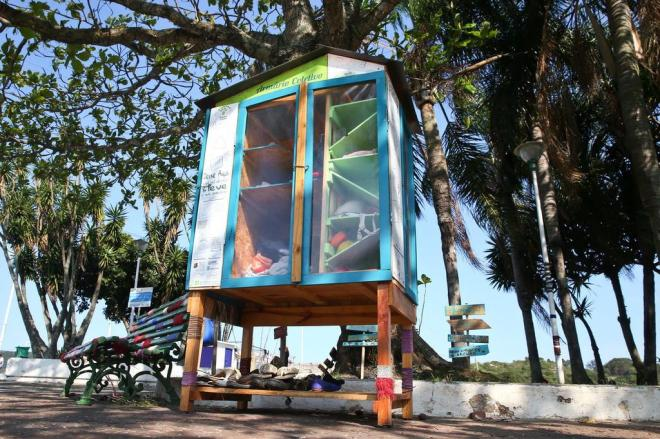
\includegraphics[width=0.7\linewidth]{produtos/prodquatro/armario_coletivo}
	\caption{Contêiner do Armário Coletivo}
	\label{fig:armario_coletivo}
	\legend{Fonte: Jornal Diário Catarinense}
\end{figure}


\newpage
\FloatBarrier
\section{Procedimentos operacionais e especificações mínimas a serem adotados nos serviços públicos de limpeza urbana e de manejo de resíduos sólidos}
\label{sec:proc_oper}
%% Manual item V
%% Entrega 1: 30.nov.2019
%% Autora: Maysa Rocha

De acordo com o item 1.2.1 Acondicionamento - produto 3, o acondicionamento de resíduos comuns no município é composto por 59 lixeiras. Os resíduos comuns domiciliares e comerciais ficam normalmente armazenados em lixeira de ferro de dimensões (2x1x1 metros) ou lixeiras de madeira de dimensões (2x1x1 metros ou 1,20x1x1 metros). A problemática inserida é que apesar das lixeiras apresentarem um volume significativo, algumas classes de resíduos são dispostas inadequadamente no solo ao lado das lixeiras. Em vista disso, para erradicar o problema, é necessário um acondicionamento que possua uma porta de entrada, de modo que facilite tanto o trabalho do catador ou do agente de limpeza, quanto do morador que deposita o lixo no local adequado. O Departamento de Meio Ambiente de Flores da Cunha realizou a instalação de novas lixeiras para coleta seletiva no município (\autoref{fig:lixeirafloresdacunha}), que possuem as características descritas.   

\begin{figure}
	\centering
	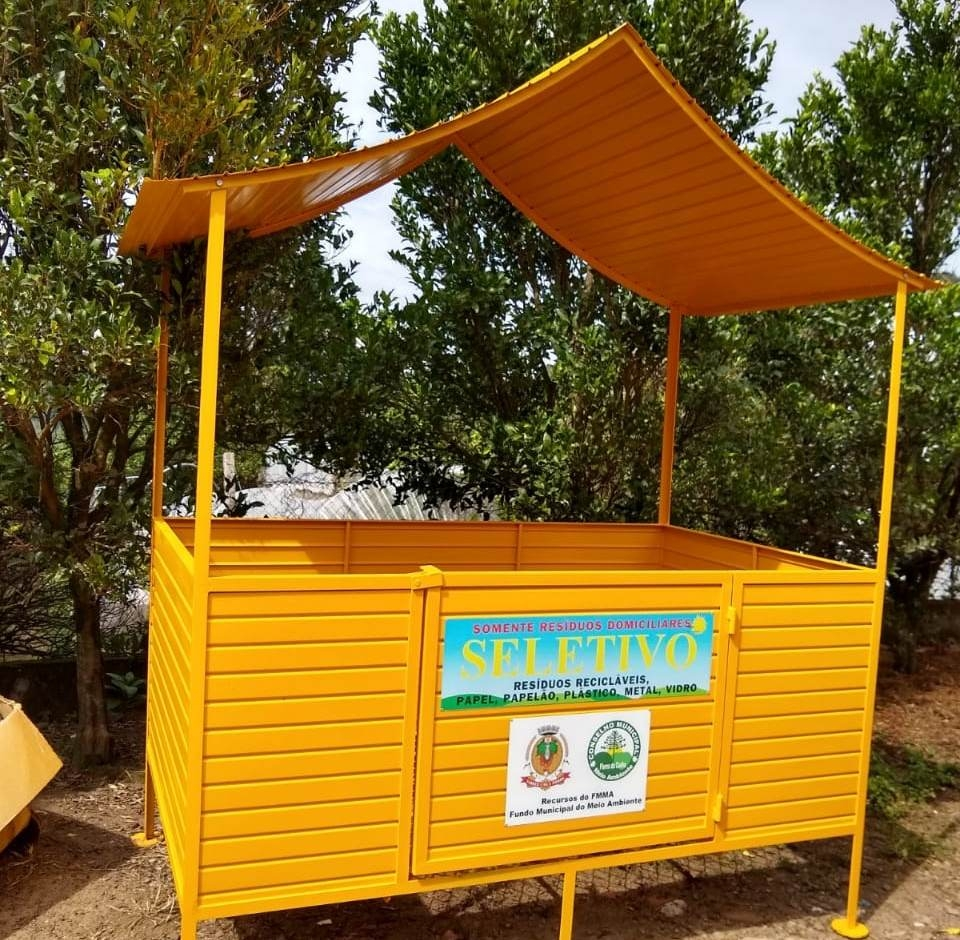
\includegraphics[width=0.7\linewidth]{produtos/prodquatro/lixeira_floresdacunha}
	\caption{Acondicionamento do município Flores da Cunha}
	\label{fig:lixeirafloresdacunha}
	\legend{Fonte: Jornal O Florense}
\end{figure}

Outras proposta interessante seria personalizar os acondicionamentos e fornecer dois para cada local ou criar uma divisória no mesmo, a fim de dividi-los entre resíduos orgânicos e recicláveis.
O Guia para elaboração dos Planos de Gestão de Resíduos Sólidos, disponibilizado pelo Ministério do Meio Ambiente discorre sobre um “Estudo de Regionalização”, que deve pré-dimensionar as instalações e sua localização adequada para a gestão dos resíduos sólidos em cada arranjo intermunicipal, tais como: pontos de entrega de resíduos, galpões de triagem dos resíduos secos, compostagem de resíduos orgânicos, instalações de tratamento dos resíduos dos serviços de saúde, aterros sanitários, aterros de resíduos da construção civil e inertes e outras instalações que permitam o manejo diferenciado e integrado dos diversos tipos de resíduos gerados na UF. Dentre as unidades e infraestruturas para a destinação final de resíduos podem ser citadas: 


\begin{itemize}
	\item LEV – Locais de Entrega Voluntária para Resíduos Recicláveis. Dispositivos de recebimento de recicláveis, como contêineres ou outros; 
	\item PEV – Pontos de Entrega Voluntária para RCC e Resíduos Volumosos, para acumulação temporária de resíduos da coleta seletiva e resíduos com logística reversa (conforme NBR 15.112/2004);
	\item Galpão de triagem de recicláveis secos; 
	Unidades de valorização de orgânicos (compostagem e biodigestão);
	\item ATT – Áreas de Triagem, Reciclagem e Transbordo de RCC, Volumosos e resíduos com logística reversa;
	\item Aterros sanitários (NBR 13.896/1997);
	\item ASPP - Aterro Sanitário de Pequeno Porte (NBR 15.849/2010); 
	\item Aterros de RCC Classe A (NBR 15.113/2004).
\end{itemize}

A Confederação Nacional de Municípios (CNM) destaca a diferença entre o Ponto de Entrega Voluntária (PEV), conhecidos também como Ecopontos, e o Local de Entrega Voluntária (LEV). PEV ou Ecoponto são locais, determinados pelas prefeituras, com equipamentos destinados para a acumulação temporária de resíduos da construção e demolição, de resíduos volumosos, da coleta seletiva e resíduos com logística reversa. Esses locais são amplos e com espaços bem definidos para cada tipo de resíduo a ser depositado no local. Os LEVs são locais de Entrega Voluntária de Resíduos Recicláveis, são contêineres, sacos ou outros dispositivos instalados em espaços públicos ou privados monitorados, para recebimento de recicláveis. A principal diferença entre eles é que os PEVs recebem resíduos volumosos e que fazem parte da logística reversa. Os LEVs são equipamentos menores, mas também aptos a armazenarem resíduos da coleta seletiva.

\newpage
\FloatBarrier
\section{Indicadores para os serviços públicos de limpeza urbana e de manejo de resíduos sólidos}
\label{sec:indicadores}
%% Manual item VI
%% Entrega X: XX.nov.2019
%% Autora: Indefinido

\newpage
\FloatBarrier
\section{Regras para o transporte e outras etapas do gerenciamento de resíduos sólidos sujeitos ao plano de gerenciamento específico}
\label{sec:regras_trans}
%% Manual item VII
%% Entrega 1: 30.nov.2019
%% Autora: Lia Yukari

Para a elaboração dessa seção, foi considerado o disposto na \gls{pnrs} (Lei Federal nº 12.305/2010) e seu regulamento (Decreto nº 7.404/2010); tão bem como diversas outras normas dispostas e referenciadas de acordo com seu respectivo tipo de resíduo.

Aos resíduos sólidos como um todo, salienta-se normas a serem usadas como referência e importante para capacitação técnica e concordância de práticas relacionadas à resíduos:

\begin{itemize}
	\item \gls{nbr} 10004/04 – Resíduos sólidos – Classificação \cite{abnt:10004:2004};
	\item \gls{nbr} 12980/93 - Coleta, varrição e acondicionamento de resíduos sólidos urbanos - Terminologia \cite{abnt:12980:1993};
	\item \gls{nbr} 7500/01 – Identificação para o transporte terrestre, manuseio, movimentação e armazenamento de produtos \cite{abnt:7500:2001}.
\end{itemize}

Para os resíduos que se classificam como resíduos perigosos (vide \cite{abnt:10004:2004}), tem-se como base as normas:

\begin{itemize}
	\item \gls{nbr} 12235/92 – Armazenamento de resíduos perigosos \cite{abnt:12235:1992};
	\item \gls{nbr} 7501/11 – Transporte terrestre de produtos perigosos – terminologia \cite{abnt:7501:2011}; 
	\item \gls{nbr} 10157/87 – Aterros de resíduos perigosos – critérios para projetos, construção e operação \cite{abnt:10157:1987}.
\end{itemize}

Com base no Diagnóstico Municipal de Monteiro Lobato (Produto 3), evidenciou-se a proeminência de quatro tipos de resíduos gerados no município. Para tais, foram levantadas as devidas normas para seu transporte adequado, desde armazenamento a disposição final. São eles:

\begin{itemize}
	\item \gls{rsu}: comum e seletivo;
	\item \gls{rcc};
	\item \gls{rss};
	\item Resíduos de Logística Reversa.
\end{itemize}

	\subsection{\gls{rsu}}
	Os \gls{rsu} compreendem os resíduos domiciliares e os resíduos de limpeza urbana. Os resíduos domiciliares são os resíduos originários de atividades domésticas em residências urbanas. Os resíduos de limpeza urbana englobam os resíduos originários de varrição, de limpeza de logradouros, de vias públicas e de capina e poda \cite{brasil:12305, brasil:11445}.
	
	No município de Monteiro Lobato os \gls{rsu} são divididos em duas categorias: resíduos sólidos comuns e resíduos sólidos recicláveis. Os resíduos sólidos comuns no município consistem em resíduos considerados domiciliares (com exceção de recicláveis), rejeitos e matéria orgânica.
	
	Os resíduos oriundos de serviços de limpeza urbana como varrição, desobstrução de sarjetas, poda e capina são usualmente considerados pelo município como resíduos comuns e recebem, em sua maioria, a mesma destinação e disposição final que os resíduos domiciliares e de estabelecimentos comerciais e prestadores de serviços.
	
	Os resíduos sólidos recicláveis são constituídos de materiais plásticos de diversas categorias, vidro, metal, papel e papelão; que possuem valor agregado e devem voltar ao sistema produtivo como matéria prima para fabricação de novos produtos através da reciclagem e/ou reaproveitamento.
	
	Atualmente, o município de Monteiro Lobato possui apenas um tipo de lixeira para o armazenamento pré-coleta, a lixeira não possui separação física para os resíduos comuns e recicláveis, podendo assim causar uma contaminação inicial caso ambos tipos de resíduos estejam dispostos concomitantemente. O município irá proporcionar novos tipos de lixeiras, e possíveis modelos encontram-se na \autoref{sec:proc_op}. %criar label na seção
	
	A coleta dos resíduos deve estar de acordo com as características dispostas na \gls{nbr} 13463 \cite{abnt:13463:1995}. Além de que, após diagnóstico realizado no município de Monteiro Lobato, é importante que haja uma política de capacitação técnica com os funcionários responsáveis pela coleta, tão bem como a disponibilizaçao de \gls{epi}. 
	
	A capacitação técnica dos funcionários também é importante quando refere-se ao transporte terrestre dos resíduos, tem-se como embasamento a \gls{nbr} 13221/03. O transporte deve ser feito por meio de equipamento adequado, obedecendo às regulamentações pertinentes \cite{abnt:13221:2003}. Atualmente, no município de Monteiro Lobato, é realizado apenas a manutenção corretiva da frota, a qual pode acarretar em uma possível paralisação temporária da coleta e transporte dos resíduos comum e reciclável. É fundamental que ocorra, com uma certa frequência, a manutenção e revisão dos meios de transporte dos resíduos, de modo preventivo; a fim de se garantir a funcionalidade dos equipamentos utilizados no gerenciamento dos resíduos sólidos.
	
	O estado de conservação do equipamento de transporte deve ser tal que, durante o transporte, não permita vazamento ou derramamento do resíduo. O resíduo, durante o transporte, deve estar protegido de intempéries,  assim como deve estar devidamente
	acondicionado para evitar o seu espalhamento na via pública ou via férrea. A descontaminação dos equipamentos de transporte deve ser de responsabilidade do gerador e deve ser realizada em local(is) e sistema(s) previamente autorizados pelo órgão de controle ambiental competente \cite{abnt:13221:2003}.
	
	O transporte sem vazamento ou derramamento deve ser garantido desde o momento de coleta até o seu local de disposição final, sendo essa disposição sem danos à saúde pública e à  segurança, tendo os seus impactos ambientais minimizados \cite{abnt:8419}. É de extrema importância listar possíveis locais para disposição final dos resíduos comuns e recicláveis, caso seja necessário o estabelecimento de uma ação emergencial, como encontra-se descrito na \autoref{sec:acoes_emerg}. %adicionar label depois
	
	
	\subsection{\gls{rcc}}
	\label{subsec:trans_rcc}
	\gls{rcc} são aqueles gerados das atividades de construções, reformas, reparos e demolições de obras de construção civil, incluindo os resíduos derivados da preparação e escavação de terrenos para obras civis, tais como: tijolos, blocos cerâmicos, concreto em geral, solos, rochas, metais, resinas, colas, tintas, madeiras e compensados, forros, argamassa, gesso, telhas, pavimento asfáltico, vidros, plásticos, tubulações, fiação elétrica, entre outros. Os \gls{rcc} são comumente denominados de entulhos de obras, caliça ou metralha \cite{brasil:12305, conama:307}. 
	
	A \gls{ssm} de Monteiro Lobato é responsável pela coleta dos \gls{rcc}. O serviço prestado pela prefeitura é taxado do solicitante através da cobrança de R\$ 41,82 por hora de serviço e por R\$ 25,09 por hora do uso do caminhão basculante. A quantidade e frequência em que ocorrem as coletas não são catalogadas internamente, dificultando assim, sua posterior análise e possíveis ações de melhoria para o manejo desse tipo de resíduo.
		
	Os \gls{rcc} gerados são armazenados na calçada em frente ao imóvel da respectiva construção civil até que seja realizada a coleta pela \gls{ssm}. Após a coleta, os \gls{rcc} são armazenados ao ar livre no pátio da prefeitura no bairro Morada do Sol,  onde observa-se a disposição inadequada dos resíduos em solo exposto e ao ar livre. Os \gls{rcc} são utilizados em estradas vicinais e nas valetas e buracos com erosões, quando necessário.
	
	Desse modo, recomenda-se o registro de cada uma das coletas, com sua respectiva data, horário, quantidade de \gls{rcc}, nome do solicitante, valor da taxa e qualquer outro tipo de informação que seja válida.
	
	Quanto ao armazenamento do \gls{rcc}, é importante a presença de uma área de transbordo adequada (bota fora regularizado); em que o resíduo não esteja exposto à chuva, sol intenso, vetores e animais. Faz-se também importante que o resíduo não esteja em contato direto com o solo, a fim de se evitar contaminações no mesmo ou em águas pluviais; para tal, recomenda-se o uso de recepientes adequados ou uma camada impermeabilizada.
	
	Ademais, o resíduo é reaproveitado no município conforme demanda dos próprios munícipes. É possível elaborar projetos de reaproveitamento dos \gls{rcc} em construções civis e também para manutenção das estradas - como é realizado atualmente; mas de modo controlado, analisado, seguro e estável.
	
	\subsection{\gls{rss}}
	Os \gls{rss} são definidos como os resíduos provenientes de atividades de atendimento à saúde humana ou animal, incluindo os serviços de assistência domiciliar e de trabalhos de campo; laboratórios analíticos de produtos para saúde; necrotérios, funerárias e serviços onde se realizem atividades de embalsamamento; serviços de medicina legal; drogarias e farmácias inclusive as de manipulação; estabelecimentos de ensino e pesquisa na área de saúde; centros de controle de zoonoses; distribuidores de produtos farmacêuticos; importadores, distribuidores e produtores de materiais e controles para diagnóstico in vitro; unidades móveis de atendimento à saúde; serviços de acupuntura; serviços de tatuagem, entre outros similares \cite{conama:362}.
	
	No município de Monteiro Lobato há a presença de uma \gls{ubs} (realiza serviço 24 horas de pronto atendimento e atendimento de ambulatório de segunda-feira à sexta-feira) e mais sete principais estabelecimentos geradores de \gls{rss} (que englobam veterinários, consultórios odontológicos, farmácia e estabelecimento de comércio de produtos para animais). 
		
	Tanto a \gls{ubs} quanto a maioria dos estabelecimentos geradores de \gls{rss} não dispõem de um \gls{pgrss}. Com base no diagnóstico elaborado, algumas defasagens relacionadas ao tratamento dos resíduos nos estabelecimentos de saúde foram identificados, tais como a segregação incorreta dos resíduos comuns e recicláveis, a forma adequada de acondicionamento do \gls{rss} de acordo com sua respectiva classe e o local de armazenamento temporário.
	
	A maioria dos estabelecimentos geradores de \gls{rss} encaminham seus resíduos à \gls{ubs} do município, a qual os armazena em um ambiente específico. A  empresa especializada AGIT Soluções Ambientais Ltda é a responsável pelo serviço de coleta (de 15 em 15 dias), transporte e incineração que ocorre no município de Itajubá. 
	
	Desse modo, é importante a presença de um \gls{pgrss}, prioritariamente a \gls{ubs} do município por acondiocionar o \gls{rss} de outros estabelecimentos. Para um correto tratamento do \gls{rss}, foi utilizado como referência o Manual da \gls{anvisa}, de 2006, apresentado no Produto 3 (diagnóstico).
	
	Ademais, acentua-se duas normas importantes ao tratar-se da capacitação técnica de funcionários dentro de um estabelecimento de saúde, definindo a terminologia em relação aos \gls{rss} e os procedimentos exigíveis para garantir condições de higiene e segurança no processamento interno de resíduos infectantes, especiais e comuns, nos serviços de saúde. São elas, respectivamente \cite{abnt:12807:1993, abnt:12809:1993}:
	
	\begin{itemize}
		\item \gls{nbr} 12807/93 – Resíduos de serviços de saúde
		\item \gls{nbr} 12809/93 – Manuseio de resíduos de saúde
	\end{itemize}
	
	Por fim, em 2018, a \gls{anvisa} - através de uma \gls{rdc} - regulamentou os requisitos de Boas Práticas de Gerenciamento dos \gls{rss}. Em seu Art. 5º, estabelece que todo serviço gerador deve dispor de um \gls{pgrss}, observando as regulamentações federais, estaduais, municipais ou do Distrito Federal \cite{anvisa:222:2018}.

	
	Em seu Art. 6º, estabelece condições mínimas ao gerador de \gls{rss}, as quais devem estar coincidentes ao \gls{pgrss}. Alguns exemplos são \cite{anvisa:222:2018}:
	
	\begin{itemize}
		\item descrever os procedimentos relacionados ao gerenciamento dos \gls{rss} quanto à geração, à segregação, ao acondicionamento, à identificação, à coleta, ao armazenamento, ao transporte, ao tratamento e à disposição final ambientalmente adequada;
		\item  estar em conformidade com a regulamentação sanitária e ambiental, bem como com as normas de coleta e transporte dos serviços locais de limpeza urbana;

		\item estar em conformidade com as rotinas e processos de higienização e limpeza	vigentes no serviço gerador de \gls{rss};
		\item descrever os programas de capacitação desenvolvidos e implantados pelo serviço gerador abrangendo todas as unidades geradoras de \gls{rss} e o setor de limpeza e conservação.
	\end{itemize}
	
	\subsection{Resíduos de Logística Reversa}
	Uma das ferramentas propostas na \gls{pnrs}, para auxiliar na busca por atingir a logística reversa, é a responsabilidade compartilhada pelo ciclo de vida dos produtos. Os fabricantes, os importadores, os distribuidores e os comerciantes têm responsabilidade no recolhimento dos produtos e dos resíduos remanescentes após o uso, assim como sua subsequente destinação final ambientalmente adequada destes resíduos \cite{brasil:12305}.
	
	No diagnóstico de resíduos sólidos realizado no município de Monteiro Lobato, foi levantada uma lista dos estabelecimentos geradores de resíduos provenientes de logística reversa. Assim, com base na responsabilidade compartilhada supracitada, cabe ao munícipio o acompanhamento e fiscalização das unidades para certificar-se que estão sendo realizadas as devidas destinações finais adequadas. 
	
	O acompanhamento pode ser realizado através da disponibilização de um funcionário, ao menos uma vez por semestre, para visita e monitoramento nos estabelecimentos listados; de modo que ocorra o controle e fiscalização dos mesmos em relação à logística reversa.
	
\newpage
\section{Definição de Responsabilidades} %quanto à implementação e operacionalização do Plano
\label{sec:def_resp}
%% Manual item VIII
%% Entrega 1: 30.nov.2019
%% Autora: Talita Guerra
	
A \gls{pnrs} estabelece o conceito de responsabilidade compartilhada pelo ciclo de vida dos produtos para a gestão e gerenciamento dos resíduos gerados nos territórios. Por responsabilidade compartilhada entende-se o "conjunto de atribuições individualizadas e encadeadas dos fabricantes, importadores, distribuidores e comerciantes, dos consumidores e dos titulares dos serviços públicos de limpeza urbana e de manejo dos resíduos sólidos, para minimizar o volume de resíduos sólidos e rejeitos gerados, bem como para reduzir os impactos causados à saúde humana e à qualidade ambiental decorrentes do ciclo de vida dos produtos" \cite{brasil:12305}.

Poder público: implementação de metas para RSU/RSS/RCC
Outros - PGRS
Poder público cobra de outros o PGRS


%	A definição das responsabilidades deve ser feita quanto à implementação e à operacionalização do Plano, incluídas as etapas dos planos de gerenciamento de resíduos a que se refere o art. 20 da Lei Federal nº 12.305/2010 a cargo do poder público. 

%	Conforme o conceito de responsabilidade compartilhada pelo ciclo de vida do produto, devem ser definidas as atribuições individualizadas e encadeadas dos fabricantes, importadores, distribuidores e comerciantes, dos consumidores e dos titulares dos serviços públicos de limpeza urbana e manejo de resíduos sólidos. 
	
\FloatBarrier
\newpage
\section{Programas e ações de capacitação técnica voltados para implementação e operacionalização do Plano}
\label{sec:capac_tec}

%% Manual item IX
%% Entrega 1: 30.nov.2019
%% Autora: Lia Yukari

Essa seção discorre sobre possibilidades de capacitação técnica àqueles envolvidos na implementação e operacionalização desse \gls{pmgirs}. No diagnóstico, pôde-se avaliar deficiências relacionadas à assistência técnica e à clareza e propagação dos conhecimentos relacionados a resíduos sólidos. Com base nisso, podem ser definidos programas e ações a serem adotados em prol de uma melhor funcionalidade desse instrumento legal.

A \autoref{tab:capacit_tec} apresenta os Programas e Ações recomendados ao município de Monteiro Lobato, referente a sua capacitação técnica, seu respectivo público-alvo, modo e frequência de implementação.

	% Table generated by Excel2LaTeX from sheet 'capacit_tec'
\begin{table}[htbp]
	\centering
	\caption{Programas e Ações de Capacitação Técnica para o Município de Monteiro Lobato}
	\resizebox{\textwidth}{!}{%
	\begin{tabular}{p{12.955em}p{12.955em}p{20.59em}}
		\rowcolor[rgb]{ .969,  .588,  .275} \textcolor[rgb]{ 1,  1,  1}{\textbf{Programas e Ações}} & \textcolor[rgb]{ 1,  1,  1}{\textbf{Público-Alvo}} & \textcolor[rgb]{ 1,  1,  1}{\textbf{Implementação}} \\
		\rowcolor[rgb]{ .992,  .914,  .851} Envolvimento do Poder Executivo Municipal com as ações estabelecidas no PMGIRS & Prefeitura e secretarias municipais que encontram-se envolvidas, direta ou indiretamente, na área de resíduos sólidos & Realização de reuniões bimestrais com todos os envolvidos (ou ao menos um representante), para definição de como as ações detalhadas no PMGIRS serão implementadas \\
		\rowcolor[rgb]{ .984,  .831,  .706} Envolvimento dos funcionários municipais com as ações estabelecidas no PMGIRS & Todos os funcionários municipais que trabalham, direta ou indiretamente, na área de resíduos sólidos & Realização de reuniões semestrais com todos os funcionários municipais e Poder Executivo, para deliberação de como as ações detalhadas no PMGIRS serão implementadas \\
		\rowcolor[rgb]{ .992,  .914,  .851} Apoio técnico de especialistas, de escolas ou universidades e de instituições voltadas à área de resíduos sólidos & Poder Executivo Municipal, funcionários e munícipes de Monteiro Lobato & Estabelecimento de parcerias com escolas, universidades ou instituições para estudo da implementação e acompanhamento trimestral da operacionalização das ações detalhadas no PMGIRS.  \\
		\rowcolor[rgb]{ .984,  .831,  .706} Envolvimento da população com as ações estabelecidas no PMGIRS & Munícipes de Monteiro Lobato & Ampla divulgação das audiências do PMGIRS. Propagação contínua do conteúdo do PMGIRS; através de informativos, mídias sociais e disseminação em eventos, instituições e escolas. \\
		\rowcolor[rgb]{ .992,  .914,  .851} Apresentação de dados na base SNIS & Prefeitura e secretarias municipais que encontram-se envolvidas, direta ou indiretamente, na área de saneamento básico & Abastecimento mensal de dados e informações do município, para controle e futura análise das ações implementadas no PMGIRS. \\
	\end{tabular}%
}
	\label{tab:capacit_tec}%
\end{table}%

	
É importante salientar que a responsabilidade de implementação e operacionalização é inteiramente do município, o qual cabe ao mesmo firmar qualquer tipo de apoio técnico que seja necessário ou conveniente. Assim, como auxílio de capacitação técnica, entende-se a disponibilidade para consultoria relacionada ao gerenciamento dos resíduos sólidos e a orientação das ações prescritas nesse Produto.

As linhas de ações principais são aquelas voltadas à educação ambiental e as preventivas e corretivas; tão bem como o cumprimento das metas de redução, reutilização, coleta seletiva e reciclagem, entre outras, com vistas a reduzir a quantidade de rejeitos encaminhados para disposição final ambientalmente adequada.

\FloatBarrier
\newpage
\section{Programas e ações de educação ambiental}
\label{sec:educ_amb}
%% Manual item X
%% Entrega X: XX.nov.2019
%% Autora: Talita Guerra e Maysa Rocha
trazer a questão dos catadores - eles conhecem o território e sua dinâmica como ninguém

reativação do conselho do meio ambiente municipal

criação de um grupo de apoio para o cumprimento das metas e dos objetivos

articulação entre os entes das sociedade para identificação de soluções individuais ou coletivas que por ventura já sejam realizadas e que possam ser replicadas ou adaptadas em outras comunidades e setores da sociedade.

estabelecer o canal de comunicação e mantê-lo aberto, horizontalmente, entre os entes.

realização de oficinas participativas com líderes comunitários

priorizar a educação ambiental nos planos de ensino escolares

cobrar educação ambiental das empresas

levar as medidas de educação ambiental para dentro do setor público


\label{sec:educ_amb}
O termo "educação ambiental" possui diversas definições e uma delas foi descrita no Congresso de Belgrado, promovido pela UNESCO em 1975, e foi compreendida como um processo que visa: “(...) formar uma população mundial consciente e preocupada com o ambiente e com os problemas que lhe dizem respeito, uma população que tenha os conhecimentos, as competências, o estado de espírito, as motivações e o sentido de participação e engajamento que lhe permita trabalhar individualmente e coletivamente para resolver os problemas atuais e impedir que se repitam (...)" 

O \gls{mma} retrata a ideia central da \gls{pnrs} como uma transformação da visão sobre os resíduos sólidos, o que antes era visto como uma reta (desde a extração da matéria prima até o "jogar o lixo fora"), agora é visto como um ciclo onde as pontas se juntam (o que antes era lixo, inútil, torna-se recurso em potencial). Esse princípio de gestão integrada de resíduos busca incorporar e denominar como responsável quem legisla, quem produz, quem consome, quem recicla e quem cuida do destino final. Em outras palavras, estabelece a responsabilidade compartilhada por todos os entes da sociedade pela geração e manejo dos resíduos sólidos. 

Essa mudança de visão sobre os resíduos muitas vezes não é imediata ou natural; o habitual é usar e descartar, afastar o que não serve mais da vista. Logo, há a necessidade de investir-se em políticas voltadas à educação ambiental com foco na transformação do pensar sobre o que é "lixo", buscando um novo olhar para os hábitos costumeiros de consumo e descarte, incentivando a criatividade como propulsora de ideias e ações para a resolução de questões relacionadas aos resíduos. 

\subsection{Objetivos}

pois irá influenciar nas atividades cotidianas e locais, por exemplo: qualidade de vida, escolhas de consumo, cultura da descartabilidade, limpeza do município, erradicação dos vetores de doenças, entre outros pontos. 

\subsection{Público-alvo}

É importante enfatizar que a educação ambiental não se restringe apenas ao âmbito escolar. Muito além que trabalha-la com crianças e jovens regularmente matriculados em instituições de ensino, a educação ambiental necessita abranger a comunidade como um todo: as crianças, seus pais e professores; as empresas e os funcionários; as comunidades de moradores; os turistas; o poder público. Logo, o público-alvo das ações voltadas à Educação Ambiental compreende toda a comunidade Lobatense. 

\subsection{Metas, projetos e ações}

\FloatBarrier
\newpage
\section{Programas e ações para a participação de grupos interessados}
\label{sec:grup_int}
%% Manual item XI
%% Entrega X: XX.nov.2019
%% Autora: Laís Shiki

\FloatBarrier
\newpage
\section{Mecanismos para a criação de fontes de negócios, emprego e renda}
\label{sec:mec_renda}
%% Manual item XII
%% Entrega X: XX.nov.2019
%% Autora: Laís Shiki

\newpage
\section{Sistema de cálculo dos custos da prestação dos serviços públicos de limpeza urbana e de manejo de resíduos sólidos}
\label{sec:calculo_custo}
%% Manual item XIII
%% Entrega X: XX.nov.2019
%% Autora: Lia Yukari

\begin{comment}

sistema de cálculo dos custos da prestação dos serviços públicos de limpeza urbana e de manejo de resíduos sólidos, bem como a forma de cobrança desses serviços, observada a Lei nº 11.445, de 2007;

(i) melhores rotas relacionada ao custo (ii) registrar dias de coleta, completa ou parcial, ida a Tremenbé ou não, fazer um controle no geral

% manual

O controle do sistema de cálculo dos custos da prestação (estrutura financeira) dos serviços públicos de limpeza urbana e de manejo de resíduos sólidos, incluindo o funcionamento da estrutura de receitas e despesas, tanto do custeio como dos investimentos em infraestrutura, obras civis, maquinário, frota de veículos, juntamente com os procedimentos relativos ao controle de custos operacionais dos serviços, das fiscalizações e das medições, dentre outros, deve produzir a alocação eficiente dos recursos.

A Lei Federal nº 11.445/2007 assegura a estabilidade econômico-financeira dos serviços de limpeza urbana e manejo de resíduos sólidos urbanos por meio de taxas ou tarifas e outros preços públicos, em conformidade com o regime de prestação do serviço ou de suas atividades.

A estrutura de remuneração e cobrança dos serviços públicos de limpeza urbana e manejo de resíduos sólidos poderá levar em consideração os seguintes fatores:
•		Categorias de usuários, distribuídas por faixas ou quantidades crescentes de utilização ou de consumo;
•		Padrões de uso ou de qualidade requeridos;
•		Quantidade mínima de consumo ou de utilização do serviço, visando à garantia de objetivos sociais, como a preservação da saúde pública, o adequado atendimento aos usuários de menor renda e a proteção do meio ambiente;
•		Custo mínimo necessário para disponibilidade do serviço em quantidade e qualidade adequadas;
•		Ciclos significativos de aumento da demanda dos serviços, em períodos distintos;
•		Capacidade de pagamento dos consumidores.
A remuneração pela prestação de serviço público de manejo de resíduos sólidos deve ainda levar em conta a destinação adequada dos resíduos coletados e pode considerar os seguintes elementos:
•		Nível de renda da população da área atendida;
•		Características dos lotes urbanos e as áreas que podem ser neles edificadas;
•		Peso ou volume médio coletado por habitante ou por domicílio;
•		Mecanismos econômicos de incentivo à minimização da geração e à recuperação dos resíduos gerados.
Na etapa de diagnóstico do PMGIRS deverá ser apresentado um panorama quanto ao sistema financeiro municipal, analisando as receitas geradas e as despesas com serviços relacionados à gestão e manejo de resíduos sólidos. Esta abordagem colaborará para o conhecimento de como a municipalidade mantém e prioriza o planejamento e a gestão das receitas, bem como os pagamentos de despesas relativas à gestão dos resíduos sólidos.
Já na etapa de prognóstico deverão ser apresentados os aspectos e exemplos referentes à cobrança pelos serviços públicos de limpeza urbana e de manejo de resíduos sólidos. Deve-se apresentar as formas de cobrança por estes serviços, a definição e proposição da melhor alternativa para o cálculo da taxa/tarifa municipal de resíduos sólidos.
Deve-se atentar para §7o do art. 33 da Lei Federal nº 12.305/2010 que trata da estruturação e implementação dos sistemas de logística reversa.
Para taxas e tarifas, os reajustes devem observar o intervalo mínimo de 12 (doze) meses e, assim como para as revisões, devem ser tornados públicos com antecedência mínima de 30 (trinta) dias com relação à sua aplicação.
Para mais informações consulte os aspectos econômicos e sociais da Lei Federal nº 11.445/2007 e do Decreto nº 7.217/2010.

\end{comment}

O controle do sistema de cálculo dos custos da prestação (estrutura financeira) dos serviços públicos de limpeza urbana e de manejo de resíduos sólidos, incluindo o funcionamento da estrutura de receitas e despesas, tanto do custeio como dos investimentos em infraestrutura, obras civis, maquinário, frota de veículos, juntamente com os procedimentos relativos ao controle de custos operacionais dos serviços, das fiscalizações e das medições, dentre outros, deve produzir a alocação eficiente dos recursos \cite{agevap_manual_2019}.

A Lei Federal nº 11.445/2007 assegura a estabilidade econômico-financeira dos serviços de limpeza urbana e manejo de resíduos sólidos urbanos por meio de taxas ou tarifas e outros preços públicos, em conformidade com o regime de prestação do serviço ou de suas atividades \cite{agevap_manual_2019}.


\newpage
\FloatBarrier
\section{Propostas para redução, reutilização, coleta seletiva e reciclagem de resíduos}
\label{sec:metas}
%% Manual item XIV
%% Entrega 1: 30.nov.2019
%% Autora: Talita Guerra

De acordo com o Diagnóstico Municipal Participativo (Produto 3), uma das fragilidades em relação a consistência de informações que sejam fidedignas à realidade do município é a não identificação e mensuração correta dos dados necessários para inserção na base federal \gls{snis}. A ausência de informações corretas a respeito dos serviços de saneamento pode impedir ou dificultar o conhecimento sobre a situação do município e o planejamento e execução de medidas de controle, mitigação ou solução das questões.

Os formulários de preenchimento do \gls{snis} são muitas vezes extensos porém bastante completos e as informações solicitadas são de conhecimento do município (contratos, registros de operações, folhas de pagamento, etc.).	A partir do preenchimento das informações, o \gls{snis} calcula indicadores de situação que podem ser utilizados para nortear as políticas públicas em relação aos serviços de saneamento básico, dentre eles o gerenciamento de resíduos sólidos, mas esses indicadores somente serão úteis se o município detiver o controle das informações prestadas. 

Em relação aos resíduos sólidos, o município deverá ter clareza da situação da geração e movimentação dos resíduos em seu território (por exemplo: quantidade total de resíduos, quantidade por classe de resíduos, flutuação da quantidade em períodos de alta temporada turística, quantidade de resíduos recicláveis, quantidade de catadores existentes, índice de atendimento de coleta urbana e rural, situação dos caminhões, dentre outras situações) para então planejar e implantar soluções que impactem positivamente na melhoria dos serviços de saneamento e consequentemente na qualidade de vida dos munícipes, tornando a gestão mais eficiente.

Ao se pensar em medidas para a diminuição dos resíduos encaminhados para disposição final ambientalmente adequada, é comum a lembrança da política dos 3Rs relacionados aos resíduos sólidos: redução, reutilização, reciclagem. De fato, a \gls{pnrs}, em seu artigo 9º, estabelece como uma de suas diretrizes a ordem de prioridade na gestão e gerenciamento de resíduos sólidos: a não geração, a redução, reciclagem, o tratamento dos resíduos sólidos e por fim a disposição ambientalmente adequada dos rejeitos. \cite{brasil:12305} Por rejeito entende-se todos os resíduos para os quais não há mais possibilidade de tratamento e recuperação, seja por ausência de tecnologia ou por não ser economicamente viável.

Como mostrado no Diagnóstico Municipal Participativo (Produto 3), boa parte dos resíduos gerados em Monteiro Lobato são passíveis de aproveitamento, o que os coloca na condição de recursos potenciais, inclusive com geração de renda e não devem, portanto, ter como destino final o aterramento. 

Neste sentido, esta seção do Prognóstico (Produto 4) apresenta algumas propostas que podem ser implantadas no município para promover a redução dos resíduos gerados e atualmente encaminhados para aterro e reaproveitamento de recursos.

\subsection{Redução da quantidade de resíduos sólidos encaminhados para disposição final}


\textbf{\underline{Para que o município consiga atingir as metas para ..... gestão, seguir os indicadores já propostos no Produto 3. Essas metas são.....}}



\subsubsection{Resíduos orgânicos}

O tratamento dos resíduos orgânicos pode ocorrer de diversas e para diversas finalidades

A compostagem é uma dessas formas e de acordo com a Lei de Saneamento Básico (Lei nº 11.445) também é considerada serviço de limpeza urbana e cabe ao titular dos servições de limpeza pública articular para a implantação de sistemas de compostagem.

A compostagem de resíduos orgânicos é a decomposição, na presença de oxigênio, da matéria orgânica dos resíduos de origem animal e vegetal, que têm sua carga orgânica neutralizada e transformada em matéria rica em nutrientes, sem odor e sem potencial poluidor, que podem ser incorporados ao solo tornando-o melhor para o desenvolvimento de plantas e pode ser vinculada a diversos benefícios socioambientais além da redução de resíduos a serem dispostos:

\begin{itemize}
	\item Redução de resíduos para aterramento, consequentemente redução de custos associados e aumento de vida útil do aterro;
	\item Produção de potencial adubo devido a reciclagem de nutrientes;
	\item Uso agrícola do adubo e diminuição dos custos financeiros associados à compra de fertilizantes e diminuição dos custos ambientais inerentes à produção desses fertilizantes;
	\item Diminuição da emissão de CH4 (metano) para a atmosfera, gás de elevado potencial de efeito estufa. 
\end{itemize}

Os materiais que podem ser compostados são diversos e geralmente são resíduos orgânicos em geral (domésticos ou não), aparas de grama, resíduos de poda e capina, cinzas e etc, e em geral a montagem de uma composteira, independentemente do tamanho é de uma mistura de parte de resíduo orgânico úmido para partes de matéria seca (serragem, grama seca, lascas de madeira e etc). A atividade pode ser implantada nos municípios desde que haja controle sobre a qualidade dos processos e do produto para que não ocorra a geração de compostos contaminados ou a atividade se torne contaminante do local \cite{felipetto_conceito_2007}. A segregação na fonte é uma das etapas mais importantes do processo de compostagem pois evita que contaminantes como medicamentos, pilhas e outros sejam misturados aos resíduos compostáveis e terminem por prejudicar a qualidade do material final. Por esse motivo é importante conscientizar a população e viabilizar a correta separação dos resíduos compostáveis de outros tipos de resíduos (recicláveis, resíduos de logística reversa, resíduos de construção civil e etc) e dos rejeitos.

Como abordado no Diagnóstico Municipal (Produto 3), cerca de 34 \% dos resíduos da coleta comum no município de Monteiro Lobato são compostos por matéria orgânica que poderia ser compostada, o que diminuiria a contribuição do município tanto em relação a quantidade de resíduos que deixaria de ser aterrada e consequentemente seus próprios custos, quanto a participação na produção de \gls{gee}. Boa parte dos moradores (cerca de 50 \%) e algumas comunidades municipais já fazem compostagem nos seus espaços próprios, a exemplo do\underline{\textbf{ bairro dos Souzas.}} O poder público local, focando na gestão participativa, poderia manter um diálogo com essas pessoas e comunidades e estabelecer parcerias para troca de informações, métodos e materiais, como equipamentos e matéria seca.

Quando realizado pelos geradores em ambiente domiciliar (no caso, os munícipes) é classificada como compostagem doméstica. Essa forma de compostagem é realizada em recipientes chamados de composteiras ou minhocários, caso sejam utilizadas minhocas no processo. A vantagem da composteira doméstica é que além de diminuir o impacto e os custos inerentes à coleta e destinação desses resíduos, proporciona o tratamento local do resíduo e produz adubo que pode ser utilizado pelo próprio munícipe em seu próprio jardim ou horta. Quando bem feita, não produz odores nem atrai animais vetores de doenças.

A compostagem também pode ser realizada através de Unidades ou Usinas de Compostagem e, neste caso, é uma atividade passível de licenciamento pelo órgão ambiental competente e que necessita ter projeto, implantação e operação bem detalhados e responsáveis técnicos. 

O Ministério do Meio Ambiente disponibilizou, em 2010, o Manual para implementação de compostagem e de coleta seletiva no âmbito de consórcios públicos. De acordo com esse manual, podem ser implementados  

%caso a compostagem seja feita pelo município, será necessário ter licença? será necessário atender todos os padrões para fazer adubo? vão doar? qual o custo de implantação? pessoal? treinamento/qualificação? onde poderá ser feito?


\subsubsection{Coleta seletiva}



\subsubsection{Logística Reversa pós-consumo}

\subsection{Traçando um paralelo}
Relacionando as ideias aqui apresentadas aos \gls{ods}, verifica-se que, direta ou indiretamente a atividade pode contribuir para atingir pelo menos 5 dos objetivos:

\begin{itemize}
	\item[\gls{ods} 2] Fome zero e agricultura sustentável. Ao promover a ciclagem de nutrientes, a compostagem fornece adubo para cultivos. Boa parte do território do município de Monteiro Lobato é área rural e passível de plantios; além disso há produtores na região que podem se beneficiar da atividade ao obter adubo de qualidade a preço baixo ou nenhum, caso a atividade seja desenvolvida na propriedade. Plantios próprios podem ajudar as pessoas a ter uma alimentação mais saudável e se corretamente manejados podem contribuir para a preservação do solo, da biodiversidade local, das águas e das tradições culturais alimentares.
	\item[\gls{ods} 4] Educação de qualidade. O item 4.7 fala da educação para o desenvolvimento sustentável e estilos de vida sustentáveis. Fazer a ciclagem de nutrientes de forma local contribui para ambos os pontos.
	\item[\gls{ods} 6] [Água potável e saneamento]. Garantir a disponibilidade de água de qualidade e em quantidade significa restaurar, manter e proteger os ecossistemas que possibilitam que a água chegue nos cursos d'água. Nesse sentido enriquecer o solo das propriedades com composto para que receba plantios teria como um dos benefícios ajudar a melhorar a qualidade dos recursos hídricos da região. Além disso ao estimular a destinação correta dos resíduos, diminuindo ou mesmo acabando com os pontos de descarte incorreto de resíduos orgânicos, diminui-se a poluição decorrente desse descarte e assim também melhora a qualidade das águas da bacia. 
	\item[\gls{ods} 11]	Cidades e comunidades sustentáveis. A compostagem pode ser feita de forma privada, como solução individual, comunitária, como solução coletiva ou pelo poder público. De toda forma a diminuição do impacto poluidor e das possibilidades de soluções que a atividade propicia contribui para o desenvolvimento de um espaço mais harmonioso e sustentável.
	\item[\gls{ods} 12] Consumo e produção responsáveis. Resíduos orgânicos, muitas vezes são provenientes do desperdício de alimentos, em toda a cadeia de produção até o consumidor final. Repensar a forma de lidar com o próprio resíduo pode fazer com que as pessoas repensem o consumo que gera o resíduo.  
\end{itemize}


\newpage
\FloatBarrier
\section{Projeções para o horizonte de 20 anos do Plano}
%% Item novo
%% Entrega 1: 30.nov.2019
%% Autora: Talita Guerra
%	https://www.mma.gov.br/estruturas/srhu_urbano/_arquivos/1_manual_elaborao_plano_gesto_integrada_rs_cp_125.pdf


%	https://www.mma.gov.br/cidades-sustentaveis/residuos-solidos/material-t%C3%A9cnico.html

%	http://www.pmf.sc.gov.br/sistemas/pmgirs/arquivos/PMGIRS_CADERNO_3_Prognostico_PMGIRS_Florianopolis.pdf

PGRSS para os estabelecimentos geradores de RSS
Descarte específico chapa de raio X
separação de resíduos na ubs 
recipientes rígidos para armazenagem dos resíduos na ubs

novamente, dificuldade para interpretar os dados devido a falta de dados consistentes

cadastro dos geradores de rss
controle dos pesos/volumes/massas dos geradores particulares, por classe de resíduo

rcc - mun: caracterizar grandes e pequenos geradores para facilitar a elaboração PGRCC

pequenos volumes: pev - troca; incentivo a recuperação de móveis (fonte de renda) - coleta e doa

informações de acesso livre

aumentar pontos de coleta de óleo - gerenciar retirada

\subsection{Projeção populacional: total, urbana, per capta}

A estimativa de crescimento populacional foi feita com base nos dados do Censo de 2010 do \gls{ibge} e utilizando o método geométrico para o crescimento das populações através de uma planilha disponibilizada pelo \gls{mma} (Planilha MMA)  %https://www.mma.gov.br/cidades-sustentaveis/residuos-solidos/material-t%C3%A9cnico.html).

% Table generated by Excel2LaTeX from sheet 'Planilha1'
\begin{table}[htbp]
  \centering
  \arrayrulecolor{white}
  \caption{Projeção da população do município de Monteiro Lobato para o horizonte de 20 anos do Plano}
    \begin{tabular}{c|c|c|c}
    \rowcolor[rgb]{ .969,  .588,  .275} \multicolumn{4}{c}{\textcolor[rgb]{ 1,  1,  1}{\textbf{Projeção populacional}}}\\
    \rowcolor[rgb]{ .984,  .831,  .706} \textbf{Ano} & \textbf{Pop. Urbana} & \textbf{Pop. Rural} & \textbf{Total} \\
    \rowcolor[rgb]{ .992,  .914,  .851} 2020  & 1.983  & 2.482  & 4.465 \\
    \rowcolor[rgb]{ .984,  .831,  .706} 2025  & 2.069  & 2.525  & 4.594 \\
    \rowcolor[rgb]{ .992,  .914,  .851} 2030  & 2.139  & 2.544  & 4.683 \\
    \rowcolor[rgb]{ .984,  .831,  .706} 2035  & 2.193  & 2.544  & 4.737 \\
    \rowcolor[rgb]{ .992,  .914,  .851} 2040  & 2.228  & 2.518  & 4.746 \\
    \end{tabular}%	
  \label{tab:proj_pop}%
  \legend{Fonte: Fundação Seade.}
\end{table}%


Caso a projeção populacional se confirme, Monteiro Lobato terá um acréscimo de aproximadamente XXXXX pessoas que devem contribuir para o aumento da geração de resíduos sólidos no município. Importante ressaltar que o próximo Censo do \gls{ibge} deverá ocorrer em breve e gerar dados populacionais mais próximos da realidade municipal, que podem diferir da projeção, ainda assim, a projeção é muito útil para fins de planejamento futuro.

\subsection{Projeção da geração de resíduos total e per capta (por classe)}

As projeções foram feitas pelo método geométrico para as classes de resíduos para as quais o município dispõe de dados, que são os resíduos comuns e os resíduos de serviços de saúde. 

%\input{./produtos/prodquatro/proj_residuos.tex}

As taxas per capta de geração de resíduos foram estimadas pelas médias de geração do período entre 2014 e 2017. Os dados dos resíduos de saúde foram estimados com base na quantidade de resíduos recolhida pela empresa especializada AGIT Soluções Ambientais Ltda para o período. Os resíduos de saúde são classificados em 5 categorias (seção xxxxx P3) e a coleta realizada pela empresa Soluções Ambientais Ltda ocorre para os grupo de resíduos A e E. Os outros grupos são recolhidos pela coleta *****comum e não são quantificados, de modo que não há informações detalhadas sobre eles*****.

Analisando as projeções, é possível estimar um aumento da geração de \gls{rss} que ultrapassaria, em 2023, a quantidade atualmente contratada de 1,8 tonelada anual de resíduo a ser coletada e disposta pela empresa especializada, ademais, os outros grupos de resíduos de \gls{rss} (B, C, E) recolhidos pela coleta comum também devem aumentar significando elevação custos para essa classe. O grupo de resíduos D geralmente é composto por resíduos passíveis de reciclagem e representa uma grande porção do total (75\% a 90\%) gerado em locais de serviços de saúde (MMA, 2011), logo, a correta segregação e destinação adequada desse grupo pode significar recuperação de parte dos recursos graças à reciclagem.   

\subsection{Cenários possíveis}

\subsubsection{Sem aplicação do Plano}

\subsubsection{Com aplicação do Plano}	


\newpage
\FloatBarrier
\section{Descrição das formas e limites da participação do poder público local na coleta seletiva, na logística reversa e de outas ações relativas à responsabilidade compartilhada pelo ciclo de vida dos produtos}
\label{sec:lim_poder_pub}
%% Manual item XV
%% Entrega 1: 30.nov.2019
%% Autora: Laís Shiki

O Art. 30° da Lei Federal 12.305/2010 institui a responsabilidade compartilhada pelo ciclo de vida dos produtos, que segundo tal artigo deve ser implementada de forma individualizada e encadeada, abrangendo os fabricantes, importadores, distribuidores e comerciantes, os consumidores e os titulares dos serviços públicos de limpeza urbana e de manejo de resíduos sólidos. Essa responsabilidade compartilhada possui como objetivos: \cite{brasil:12305} 

\begin{itemize}
	\item Compatibilizar interesses entre os agentes econômicos e sociais e os processos de gestão empresarial e mercadológica com os de gestão ambiental, desenvolvendo estratégias sustentáveis;
	\item Promover o aproveitamento dos resíduos sólidos, direcionando-os para a sua cadeia produtiva ou para outras cadeias produtivas;
	\item Reduzir a geração de resíduos sólidos, o desperdício de materiais, a poluição e os danos ambientais;
	\item Incentivar a utilização de insumos de menor agressividade ao meio ambiente e de maior sustentabilidade;
	\item Estimular o desenvolvimento de mercado, a produção e o consumo de produtos derivados de materiais reciclados e recicláveis;
	\item Propiciar que as atividades produtivas alcancem eficiência e sustentabilidade;
	\item Incentivar as boas práticas de responsabilidade socioambiental.    
\end{itemize}

Cabe a este \gls{pmgirs}/Monteiro Lobato descrever as formas e limites da participação do poder público municipal na coleta seletiva e na logística reversa, obedecendo a \gls{pnrs} e outras legislações pertinentes ao assunto. 

\subsection{Coleta seletiva}

Implementar a coleta seletiva é essencial para atingir a meta de disposição final ambientalmente adequada dos rejeitos, segundo o Art. 9°, parágrafo um do Decreto Federal nº 7.404/2010. A Prefeitura de Monteiro Lobato já possui um sistema de coleta seletiva, que realiza coleta uma vez por semana e abrange toda a área urbana e rural do município. Na \autoref{sec:educ_amb} são propostas oficinas e ações que irão conscientizar e incentivar os munícipes e servidores públicos em relação a este sistema. 

Novamente no Art. 9° do Decreto Federal nº 7.404/2010, o parágrafo dois estabelece que a coleta seletiva deverá ser implantada pelo titular do serviço público de limpeza urbana e manejo de resíduos sólidos. Porém, o poder público local deve desenvolver ações e metas para dar continuidade na efetividade e aprimoramento do sistema de coleta seletiva. Para tanto, na \autoref{tab:limites_coleta_seletiva} são listadas algumas medidas cabíveis. 

% Table generated by Excel2LaTeX from sheet 'limites_coleta_seletiva'
\begin{table}[htbp]
  \centering
  \caption{Descrição das formas e limites da participação do poder público local na coleta seletiva}
    \begin{tabular}{P{40.855em}}
    \rowcolor[rgb]{ .992,  .914,  .851} Implantar e operar um LEV para entrega voluntária de recicláveis \\
    \rowcolor[rgb]{ .984,  .831,  .706} Estabelecer a forma correta de segregação dos RD e RC \\
    \rowcolor[rgb]{ .992,  .914,  .851} Determinar os procedimentos para o acondicionamento e descarte adequado dos materiais recicláveis \\
    \rowcolor[rgb]{ .984,  .831,  .706} Incentivar a população a realizar às boas práticas em relação a coleta seletiva \\
    \rowcolor[rgb]{ .992,  .914,  .851} Criar e priorizar a participação de cooperativas ou outro tipo de associação de catadores constituídas por pessoas físicas de baixa renda \\
    \rowcolor[rgb]{ .984,  .831,  .706} Capacitar os servidores públicos e atores sociais envolvidos na coleta seletiva \\
    \rowcolor[rgb]{ .992,  .914,  .851} Disponibilizar lixeiras específicas para cada tipo de material reciclável em pontos estratégicos no município \\
    \rowcolor[rgb]{ .984,  .831,  .706} Formentar a implementação de soluções consorciadas ou compartilhadas com municípios vizinhos \\
    \end{tabular}%
  \label{tab:limites_coleta_seletiva}%
  \legend{Fonte: Elaborado pelos autores, adaptado da PNRS (2010).}
\end{table}%


O poder público de Monteiro Lobato pode criar incentivos econômicos para os consumidores que participam da coleta seletiva, na forma de lei municipal, de acordo com o Art. 35 da \gls{pnrs}. Todavia, os consumidores possuem as seguintes obrigatoriedades:

\begin{itemize}
	\item Acondicionar adequadamente e de forma diferenciada os resíduos sólidos gerados; 
	\item Disponibilizar adequadamente os resíduos sólidos reutilizáveis e recicláveis para coleta ou devolução.    
\end{itemize}

\subsection{Logística reversa}
\label{subsec:desc_lr}

Os fabricantes, importadores, distribuidores e comerciantes de produtos obrigados a estruturar e implementar uma cadeia de logística reversa, citados na \autoref{sec:rs_geradores_lr}, devem fazer isto de forma independente do serviço público de limpeza urbana e de manejo dos resíduos sólidos \cite{brasil:12305}. Porém, é interessante o poder público local realizar certas medidas a fim de incentivar e/ou facilitar a efetivação desses sistemas. Na \autoref{tab:limites_log_reversa} são descritas algumas formas e limites para o poder público atuar nestes casos.


% Table generated by Excel2LaTeX from sheet 'limites_log_reversa'
\begin{table}[htbp]
	\centering
	\caption{Descrição das formas e limites da participação do poder público local na logística reversa}
	\begin{tabular}{P{40.855em}}
		\rowcolor[rgb]{ .992,  .914,  .851} Identificar os resíduos e seus geradores sujeitos ao sistema de logística reversa \\
		\rowcolor[rgb]{ .984,  .831,  .706} Incentivar o setor privado para a estruturação de acordos setoriais, com vista à implementação ou expansão da logística reversa \\
		\rowcolor[rgb]{ .992,  .914,  .851} Prever a participação de entidades, cooperativas de catadores ou outras formas de associações constituídas por pessoas de baixa renda na estruturação de acordos setoriais \\
		\rowcolor[rgb]{ .984,  .831,  .706} Celebrar termos de compromisso junto aos fabricantes, distribuidores e/ou comércios, visando à implantação ou expansão da logística reversa \\
		\rowcolor[rgb]{ .992,  .914,  .851} Implantar a logística reversa via promulgação de regulamentos normativos veiculados por Decreto editado pelo Poder Executivo, exigindo e fiscalizando a sua efetividade \\
		\rowcolor[rgb]{ .984,  .831,  .706} Exigir que todos os atores envolvidos no sistema de logística reversa disponibilizem informações completas sobre a realização de suas ações, com periodicidade semestral  \\
		\rowcolor[rgb]{ .992,  .914,  .851} Articular, coordenar, promover e supervisionar programas de educação ambiental com foco na logística reversa \\
		\rowcolor[rgb]{ .984,  .831,  .706} Articular com os fabricantes no sentido de implantar sistemas de logística reversa, bem como difundir tais programas \\
		\rowcolor[rgb]{ .992,  .914,  .851} Manter sistemas de logística reversa implementados em entidades e/ou instituições públicas \\
		\rowcolor[rgb]{ .984,  .831,  .706} Garantir a continuidade e permanência do processo educativo \\
		\rowcolor[rgb]{ .992,  .914,  .851} Fiscalizar o descarte ambientalmente correto dos resíduos sujeitos à logística reversa \\
	\end{tabular}%
	\label{tab:limites_log_reversa}%
	\legend{Fonte: Elaborado pelos autores, adaptado do PMGIRS/Arujá (2018)}
\end{table}%


\FloatBarrier


A fim de implementar e operacionalizar os sistemas de logística reversa, a \gls{pnrs} define os seguintes instrumentos: regulamentos, acordos setoriais e termos de compromisso, os dois últimos a serem firmados entre o poder público e o setor empresarial. Os acordos setoriais são “atos de natureza contratual, firmados entre o Poder Público e os fabricantes, importadores, distribuidores ou comerciantes, visando à implantação da responsabilidade compartilhada pelo ciclo de vida do produto” \cite{brasil:12305}. Já os termos de compromisso, ainda segundo a  \gls{pnrs}, podem ser assinados somente nos casos onde não houver acordo setorial ou regulamento específico com a mesma abrangência geográfica ou para estabelecer metas e compromissos mais exigentes que os previstos nos acordos ou regulamentos.


\newpage
\section{Meios a serem utilizados para controle e fiscalização, no âmbito local, da implementação e operacionalização dos planos de gerenciamento de resíduos sólidos e dos sistemas de logística reversa}
\label{sec:meios_controle_fisc}
%% Manual item XVI
%% Entrega 2: 13.nov.2019
%% Autora: Laís Shiki

Na \autoref{sec:rs_geradores_lr} foi identificado os resíduos sólidos e geradores que estão sujeitos ao \gls{pgrs} ou ao sistema de logística reversa em Monteiro Lobato. Neste sentido, este tópico visa propor algumas ações e indicadores para acompanhar, controlar e fiscalizar tais agentes.

Uma das ações recomendadas, para o poder público local, é a de estimar a quantidade de resíduos sujeitos ao plano de gerenciamento ou ao sistema de logística reversa.  Assim, como manter atualizado o levantamento destes geradores, é recomendado conter neste levantamento os seguintes dados: \cite{agevap_manual_2019}

\begin{itemize}
	\item Identificação do gerador: razão social, CNPJ, descrição da atividade, responsável legal, entre outras;
	\item Identificação dos resíduos gerados: resíduo, classificação, acondicionamento e/ou armazenagem, frequência de geração, entre outros; 
	\item Plano de movimentação dos resíduos: tipo de resíduo, quantidade, local de estocagem temporário (se for o caso), transporte a ser utilizado, destinação final, entre outros;
	\item Indicador de coleta: relação entre quantidade de material coletado e a quantidade de material gerado;
	\item Indicador de rejeito: relação entre o rejeito acumulado e o material recebido para tratamento.
\end{itemize}

É necessário que o município realize a cobrança do \gls{pgrs}, estipulando prazo máximo a sua entrega e penalidades caso ocorra atraso ou não execução. Vale ressaltar que aqueles que devem elaborar o \gls{pgrs} são obrigados a disponibilizar e manter atualizadas todas informações sobre a implementação e operacionalização do plano ao órgão municipal competente \cite{brasil:12305}. 

Como foi apontado no Produto 3 (Diagnóstico Municipal Participativo) deste \gls{pmgirs}, há certas irregularidades em relação ao sistema de logística reversa no município. Logo, convocar uma reunião de caráter obrigatório com comerciantes e outros envolvidos com produtos sujeitos a realizar a logística reversa, a fim de conscientizar estes sobre a importância de se elaborar o \gls{pgrs}, seria de demasiada importância. 

Utilizar os indicadores propostos no subtópico 2.6 do Produto 3 deste plano, por exemplo os indicadores para \gls{rss}, \gls{rcc} e \gls{ra}, é um meio de controlar e consequentemente fiscalizar os planos de gerenciamento e os sistemas de logística reversa.



\FloatBarrier
\newpage
\section{Ações preventivas e corretivas}
\label{sec:acoes_prev_corr}
%% Manual item XVII
%% Entrega 2: 13.nov.2019
%% Autora: Lia Yukari

Este capítulo pretende descrever as medidas preventivas e corretivas a serem adotadas pelo município quanto ao gerenciamento dos resíduos sólidos, denotando as preventivas como aquelas medidas necessárias a evitar que um problema potencial se materialize e as corretivas as ações que convergem para que um problema existente não
tenha recorrência e/ou que seu impacto seja mitigado e/ou até revertido conforme possibilidades aplicáveis ao caso concreto \cite{pmgirs_aruja3_2018}.

Qualquer atividade realizada, mesmo que planejada, está sujeita à imprevisibildades; para isso, elaborou-se nesse presente produto a \autoref{sec:emerg_corr}. As ações aqui descritas, de prevenção e correção, têm a intenção de minimizar essas ocorrências através de medidas protocoladas dentro do município em questão.

As ações preventivas e corretivas referentes ao município de Monteiro Lobato já foram descritas no Produto 3 desse presente \gls{pmgirs}, cabe ao Produto 4 delimitar os pontos práticos a serem planejados no município a fim de se concretizar tais ações de modo mais eficiente. A \autoref{tab:acoes_prevent} mostra os pontos a serem planejados e colocados em prática no município.

% Table generated by Excel2LaTeX from sheet 'acoes_prevent'
\begin{table}[htbp]
	\centering
	\caption{Ações preventivas e corretivas do município de Monteiro Lobato.}
	\resizebox{\textwidth}{!}{%
    \begin{tabular}{p{18em}p{7.91em}p{21.545em}p{21.545em}}
	\rowcolor[rgb]{ .969,  .588,  .275} \textcolor[rgb]{ 1,  1,  1}{\textbf{AÇÃO}} & \textcolor[rgb]{ 1,  1,  1}{\textbf{PRVENTIVA (P) CORRETIVA (C)}} & \textcolor[rgb]{ 1,  1,  1}{\textbf{DIAGNÓSTICO}} & \textcolor[rgb]{ 1,  1,  1}{\textbf{PROGNÓSTICO}} \\
	\rowcolor[rgb]{ .992,  .914,  .851} Controle de emissão de gases e percolados & P     & Existente. Atualmente a disposição final dos resíduos sólidos ocorre no aterro sanitário de Tremembé, dotado de sistema de drenagem e correto tratamento/destinação dos gases e percolados, de maneira a prevenir possíveis impactos advindos dos mesmos. & Fazer frequentemente o monitoramente do aterro sanitário em que são enviados os resíduos sólidos, quanto ao licenciamento exigido pelo seu respectivo Órgão Ambiental. Analisar previamente a existência de um protocolo legal caso os resíduos sólidos passem a ser dispostos em um novo local. \\
	\rowcolor[rgb]{ .984,  .831,  .706} Educação ambiental para redução e reaproveitamento de resíduos nas fontes geradoras & P     & Existente. Nas redes de ensino. O Instituto Pandavas, localizado no Bairro do Souza, é um dos principais centros pedagógicos atuantes na região. & Tornar uma ação de caráter também corretivo. Ampliar para todas as redes de ensino, instituições, empresas e comércio. Seguir aplicação de ações propostas na \autoref{sec:educ_amb}. \\
	\rowcolor[rgb]{ .992,  .914,  .851} Coleta seletiva e triagem dos resíduos & P     & Indefinido no período de elaboração desse produto. A coleta setetiva e sua triagem evita que parte dos resíduos secos recicláveis sejam destinados aos aterros sanitários. & Seguir diretrizes da \autoref{sec:capac_tec} e \autoref{sec:metas}. Melhorar a eficiência do programa de coleta seletiva. Transmitir conscientização à população quanto a separação dos resíduos recicláveis. Contar com dispositivos de entrega dos resíduos secos, como em \gls{lev}. Estabeleber um termo contratual com algum local de destinação de resíduos recicláveis. Viabilizar, antecipadamente, um termo de renovação ou uma nova associação. Levantar um cadastro de locais passíveis a receberem resíduos recicláveis em caso de emergência. \\
	\rowcolor[rgb]{ .984,  .831,  .706} Entrega voluntária de resíduos & P     & Existente. Para óleos de cozinha, evitando a destinação incorreta. Os dois pontos de entrega ocorrem através de bombonas de 50 litros e localizam-se próximos ao Terminal Rodoviário e na Secretária de Meio Ambiente e Agricultura. & Aumentar a diversidade, capacidade e abrangência dos \gls{lev} e Ecopontos a serem instalados no município, visando aumentar o atendimento à população. Realizar programas para sensibilizar a população da importância da entrega voluntária dos resíduos produzidos. \\
	\rowcolor[rgb]{ .992,  .914,  .851} Manutenção preventiva de frota e equipamentos utilizados nos serviços de limpeza e disposição final de resíduos & P/C   & Inexistente. A existência de manutenção preventiva da frota e dos equipamentos utilizados no sistema de limpeza urbana e manejo de resíduos sólidos evita situações de paralização dos serviços. & Realizar revisão preventiva nos caminhões com vistas a evitar interrupções na prestação de serviço devido a problemas mecânicos. Possuir veículos reserva os opcões pré-estabelecidas de empréstimo a fim de garantir que a prestação dos serviços de coleta e disposição final de resíduos não seja afetada por problemas na frota e interrupção da circulação de um dos caminhões. Ter disponibilidade de mecânico para realizar as manutenções necessárias e/ou convênio com alguma oficina mecânica que preste este tipo de serviço periodicamente. \\
	\rowcolor[rgb]{ .984,  .831,  .706} Programa de monitoramento da eficiência dos serviços de coleta e limpeza publica & P/C   & Inexistente. Identifica problemáticas decorrentes das estruturas e serviços, possibilitando seus devidos diagnósticos e correções, acarretando em uma maior eficiência dos serviços. & Seguir diretrizes da \autoref{sec:proc_oper}, \autoref{sec:capac_tec}, \autoref{sec:grup_int} e\autoref{sec:metas}. \\ 
	\rowcolor[rgb]{ .992,  .914,  .851} Programa de monitoramento da eficiência da disposição final de resíduos sólidos & P/C   & Inexistente. O aterro de disposição (Tremembé) contabiliza a quantidade de resíduo recebida e aterrada, porém, o município não monitora as devidas quantidades, a fim de se obter uma maior eficiência. & Seguir diretrizes da \autoref{sec:capac_tec} e \autoref{sec:metas}. Melhorar a eficiência do programa de coleta comum. Transmitir conscientização à população quanto a separação dos resíduos comuns e orgânicos. Monitorar as quantidades de resíduo aterrada por mês, tanto como catalogá-los no \gls{snis}. Viabilizar, antecipadamente, um termo de renovação com o atual local de disposição final ou uma nova associação. Levantar um cadastro de locais passíveis a receberem resíduos comuns em caso de emergência. \\
	\rowcolor[rgb]{ .984,  .831,  .706} Programa de monitoramento de descarte de RCC & P/C   & Inexistente. Identifica problemáticas decorrentes das estruturas e serviços, possibilitando seus devidos diagnósticos e correções, acarretando em uma maior eficiência dos serviços. & Regularizar um local de destinação correta dos \gls{rcc}, através de um bota fora. Realizar o controle do \gls{rcc} e seu respectivo local de acordo com a \autoref{subsec:trans_rcc}. \\
	\rowcolor[rgb]{ .992,  .914,  .851} Programa de monitoramento de geradores de Logística Reversa & P/C   & Inexistente. Identifica problemáticas decorrentes das estruturas e serviços, possibilitando seus devidos diagnósticos e correções, acarretando em uma maior eficiência dos serviços. & Garantir a funcionalidade da logística reversa através de um monitoramento de seus geradores, levantados no Produto 3. Seguir diretrizes estabelecidas na \autoref{subsec:desc_lr}. \\
	\rowcolor[rgb]{ .984,  .831,  .706} Levantamento dos geradores sujeitos aos planos de gerenciamento de resíduos sólidos e ao estabelecimento de sistemas de logística reversa. & P     & Existente. O cadastro foi realizado para a elaboração do diagnóstico do PMGIRS. Facilita a fiscalização contribuindo para que sejam evitadas práticas incorretas e consequentemente prevenindo impactos adversos decorrentes do inadequado manejo dos resíduos sólidos. & Garantir a funcionalidade da logística reversa através de um monitoramento de seus geradores, levantados no Produto 3. Seguir diretrizes estabelecidas na \autoref{subsec:desc_lr}. \\
	\rowcolor[rgb]{ .992,  .914,  .851} Cadastro de aterros próximos para uma possível recepção dos resíduos comuns em caso de impeditivo de disposição final no local atualmente utilizado & P     & Há o conhecimento acerca dos empreendimentos existentes passíveis de atender o município, podendo ser uma alternativa em caso de necessidade, mas não há contratos emergenciais pré-estabelecidos. & Estabelecer contratos emergenciais conforme descritos em \autoref{sec:emerg_corr}. Fazer uso das diretrizes estabelecidas na \autoref{sec:sol_cons} e na \autoref{sec:grup_int}. \\
	\rowcolor[rgb]{ .984,  .831,  .706} Cadastro de empresas que prestam serviços de limpeza, coleta e disposição final de resíduos como opção de contratos emergenciais para suprir uma ausência não prevista dos serviços & P     & Há o conhecimento acerca das empresas existentes passíveis de atender o município, podendo ser uma alternativa em caso de necessidade, mas não há contratos emergenciais pré-estabelecidos. & Estabelecer contratos emergenciais conforme descritos em \autoref{sec:emerg_corr}. Fazer uso das diretrizes estabelecidas na \autoref{sec:sol_cons} e na \autoref{sec:grup_int}. \\
\end{tabular}%
}
	\label{tab:acoes_prevent}%
	\legend{Fonte: Elaborado pelos autores, adaptado do PMGIRS/Arujá (2018).}
\end{table}%

\FloatBarrier

\newpage
\section{Identificação dos passivos ambientais relacionados aos resíduos sólidos e medidas saneadoras}
\label{sec:passivos_amb}
%% Manual item XVIII
%% Entrega 2: 13.nov.2019
%% Autora: Lia Yukari

Passivos ambientais são os custos (financeiros, econômicos, sociais, entre outros) necessários para preservar, recuperar e proteger o meio ambiente. A identificação do passivo ambiental diz respeito não só à sanção a ser aplicada por um dano já realizado ao meio ambiente, mas também a medidas de prevenção de danos ambientais que têm reflexos econômico-financeiros \cite{agevap_manual_2019}.

Alguns passivos ambientais relacionados aos resíduos sólidos são: Contaminação de áreas, inclusive lixões e aterros controlados; Emissão de gases; Contaminação de águas superficiais e subterrâneas \cite{agevap_manual_2019}.

\subsection{\gls{rsu}}
Em Monteiro Lobato, ocorre atualmente a disposição final adequada do \gls{rsu} em aterro sanitário com controle de emissão de gases e percolado. De qualquer forma, é sempre cabível ao município a aplicação da \autoref{sec:metas} (Metas de redução, reutilização, coleta seletiva e reciclagem) para minimizar seu impacto no aterro sanitário de destinação.

Salienta-se que, mesmo que o aterro sanitário de Tremembé esteja dentro das condições legalmente exigidas, ou não esteja localizado dentro do município de Monteiro Lobato (onde os resíduos são gerados), cabe ao município a minimização de seu impacto até a disposição final. Isso é, uma vez que os aterros sanitários contam com uma vida útil limitada, o município pode e deve reduzir ao máximo o volume a ser destinado, através de campanhas de reutilização e conscientização de separação dos recicláveis.

Ademais, a lavagem dos caminhões de \gls{rsu} (comum e reciclável) deve ser realizada de forma a não contaminar as águas superficiais e subterrâneas, sendo aderida ao sistema de esgotamento sanitário. Deve-se tomar cuidado quanto à superfície que é atingida pela água contaminada de lavagem e à rota de escoamento do mesmo, até atingir a macro drenagem.


\subsection{\gls{rcc}}
Tratando-se do \gls{rcc}, como descrito no Produto 3 e na \autoref{subsec:trans_rcc} desse Produto 4, a disposição do mesmo não é realizada de maneira adequada. Os \gls{rcc} são armazenados ao ar livre no pátio da prefeitura no bairro Morada do Sol,  onde observa-se a disposição inadequada dos resíduos em solo exposto e ao ar livre, sendo utilizados em estradas vicinais e nas valetas e buracos com erosões, quando necessário. A \autoref{fig:patio_rcc} e a \autoref{fig:rcc} mostram, respectivamente, o local e um ponto onde ocorre essa irregularidade.

\begin{figure}[h]
	\centering
	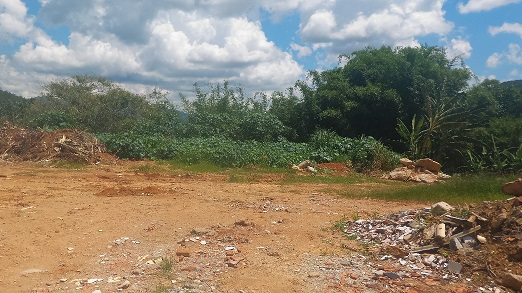
\includegraphics[width=0.7\linewidth]{produtos/prodquatro/patio_rcc}
	\caption{Pátio da Prefeitura onde são dispostos os \gls{rcc}}
	\label{fig:patio_rcc}
	\legend{Fonte: Elaborado pelos autores.}
\end{figure}

\begin{figure}[h!]
	\centering
	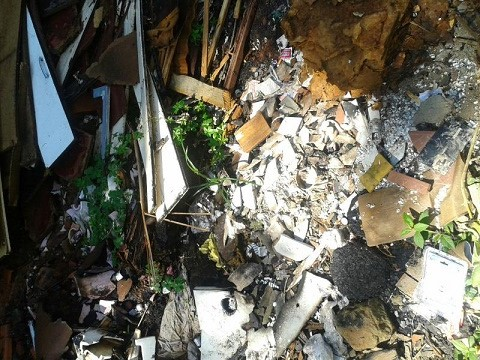
\includegraphics[width=0.6\linewidth]{produtos/prodquatro/rcc}
	\caption{Disposição inadequeda dos \gls{rcc}}
	\label{fig:rcc}
	\legend{Fonte: Elaborado pelos autores.}
\end{figure}

Dessa forma, é importante estabelecer as diretrizes propostas na \autoref{subsec:trans_rcc}, cumprindo também o papel de ação preventiva e corretiva (\autoref{tab:acoes_prevent}) desse tipo de resíduo quanto à contaminação do solo, das águas pluviais, à dispersão de vetores ou de particulados



\FloatBarrier
\newpage
\section{Periodicidade da revisão do PMGIRS}
\label{sec:revisao_pmgirs}
%% Manual item XIX
%% Entrega X: XX.nov.2019
%% Autora: Todas

\FloatBarrier
\newpage
\section{Ações para mitigação das emissões dos gases de efeito estufa}
\label{sec:acoes_efeito_estufa}
%% Manual item XX
%% Entrega 2: 13.nov.2019
%% Autora: Maysa Rocha

Segundo o relatório de Estimativas Anuais de Emissões de Gases do Efeito Estufa, realizado pelo Ministério da Ciência, Tecnologia e Inovação (2013), em 2010 o setor de disposição de resíduos sólidos e o tratamento de efluentes foi responsável por cerca de 4 \% das emissões nacionais de GEE’s.
Sendo que, as variações percentuais acumuladas no período de 2005 a 2010 mostram que as emissões desse setor cresceram a uma taxa superior a 16 \%, representando um importante setor em termos de potencial de redução de emissão

A sessão 5 do produto 3 discorre sobre a definição dos gases do efeito estufa e de forma sucinta aborda algumas ações como proposta para o município mitigar a geração dos gases do efeito estufa. 

\textbf{Rotas de coleta}
O itinerário de coleta é o trajeto que o veículo coletor deve percorrer dentro de um mesmo setor, num mesmo período, transportando o máximo de lixo num mínimo de percurso improdutivo, com o menor desgaste possível para a guarnição e o veículo. Dá-se o nome de percurso improdutivo aos trechos em que o veículo não realiza coleta, servindo apenas para o deslocamento de um ponto a outro.\cite{dalmeida_manual_2018}

Para traçar uma rota de coleta é necessário estudar alguns aspectos do meio físico da região, como por exemplo o relevo, a geomorfologia, o uso e ocupação do solo. A rota de coleta precisa ser eficiente para que percorra o menor caminho e recolha a maior quantidade de resíduos dispostos. É de suma importância pois além de diminuir gastos desnecessários com combustível, reduz a emissão de gases do efeito estufa.

\textbf{Doação de mudas}
De acordo com o relatório divulgado pela Indústria Brasileira de Árvores (Ibá), o plantio de mudas traz vantagens para o meio ambiente, principalmente no combate ao aumento da concentração dos gases do efeito estufa.
A compensação por meio de plantios florestais é uma forma
natural de sequestrar o gás carbônico pelos vegetais
através da fotossíntese, fixando-o em forma de matéria
lenhosa ou biomassa. O sequestro de carbono constitui o
processo de crescimento dos vegetais, ou seja, quanto
maior o porte da planta, mais biomassa se acumula e,
consequentemente, maior é a quantidade de carbono fixada \cite{changman_sequestroc_2004} 
Portanto, incentivar o plantio de mudas ou a doação de mudas é uma iniciativa que beneficia diretamente o meio ambiente e reduz as emissões dos gases do efeito estufa.


\textbf{Aumentar a fiscalização da queima de resíduos}
Embora, em termos globais, a queima de combustíveis fósseis (na produção de energia, nos processos industriais e nos transportes) seja a principal fonte de GEE, responsáveis pelas alterações no clima, os resíduos sólidos têm um papel importante nesse cenário, uma vez que também contribuem para a emissão desses gases \cite{IPCC_2008}. O gerenciamento inadequado dos resíduos sólidos urbanos gera diretamente outros impactos importantes, tanto ambientais quanto na saúde da população. \cite{WHO_Europe_2007}

Há também a emissão de partículas e outros poluentes atmosféricos, diretamente pela queima de lixo ao ar livre ou pela incineração de dejetos sem o uso de equipamentos de controle adequados. De modo geral, os impactos dessa degradação estendem-se para além das áreas de disposição final dos resíduos, afetando toda a população.\cite{Gouveia_riscogee_2010}

Com isso, uma proposta para erradicar a queima de resíduos sólidos  seria aumentar ou firmar a fiscalização nas ruas, em terrenos baldios para que isso não ocorra, pois a toxicidade dos gases  traz danos à saúde da população e colabora para poluição do ar.

\textbf{Redução do resíduo orgânico}
Segundo \cite{Inacio2010} a compostagem por processo aeróbico gera baixas quantidades de metano por tonelada de resíduos orgânicos em comparação com formas de tratamento anaeróbio ou disposição em aterro. Desta forma, a compostagem de resíduos apresenta grande potencial como estratégia de mitigação das emissões de metano, mesmo no contexto de amplos sistemas de gestão de resíduos urbanos, agrícolas ou agroindustriais.
Com isso, os resíduos orgânicos biodegradáveis que normalmente são dispostos inapropriadamente e são decompostos de forma anaeróbica (emissão de GEE’s), seriam tratados em um sistema aeróbio (compostagem). O uso de composto orgânico pode reduzir a dependência do uso de fertilizantes nitrogenados, que são responsáveis pela emissão de N$_{2}$O, que possui GWP(Potencial de aquecimento global) 310 vezes maior ao do CO$_{2}$. \cite{IPCC_2008}
Além da compostagem, "o município de Monteiro Lobato pode incentivar a população e os restaurantes da cidade a não desperdiçarem alimentos nas refeições, evitando sobras e utilizar todos os componentes dos mantimentos que normalmente são jogados fora, como casca, talos" e folhas, como discorre a sessão 5 do produto 3


\FloatBarrier
\newpage
\section{Ações para emergência e contingência}
\label{sec:emerg_corr}
%% Manual item XXI
%% Entrega 2: 13.nov.2019
%% Autora: Maysa Rocha

A Seção 6 do produto 3 aborda toda a parte teórica e a definição sobre ações de emergência e contingência. Este capítulo apresenta formas de como proceder em situações eventuais que impactam de alguma forma, negativa, o serviço de limpeza urbana e o manejo dos resíduos sólidos do município de Monteiro Lobato. Essas ações irão auxiliar e fornecer mais segurança, tanto à população, quanto aos prestadores de serviço, para que saibam agir da melhor forma quando ocorrer um imprevisto. Além disso, a proposta busca elevar o grau de de continuidade e de segurança dos serviços operacionais e da estrutura disponível.

A \autoref{tab:acoes_emerg_cont} apresenta algumas possíveis ocorrências do dia-a-dia e ações de emergência e contingência que podem ser tomadas para suprir o problema temporariamente.

% Table generated by Excel2LaTeX from sheet 'acoes_emerg_cont'
\begin{table}[htbp]
	\centering
	\caption{Ações de emergência e contigência para  município de Monteiro Lobato}
 	 \resizebox{\textwidth}{!}{%
	
	\begin{tabular}{p{11.275em}p{11.275em}p{25.545em}}
		\rowcolor[rgb]{ .969,  .588,  .275} \textcolor[rgb]{ 1,  1,  1}{\textbf{Ocorrência}} & \textcolor[rgb]{ 1,  1,  1}{\textbf{Origem}} & \textcolor[rgb]{ 1,  1,  1}{\textbf{Ações de emergência e contingência}} \\
		\rowcolor[rgb]{ .992,  .914,  .851} Inoperância do caminhão de resíduos & Falha na parte mecânica & · Providenciar imediatamente o reparo do equipamento\newline{}· Contatar outro município para ver a disponibilidade do caminhão de recolher os resíduos de Monteiro Lobato (rotas em comum)\newline{}· Realizar manutenção preventiva no veículo coletor \\
		\rowcolor[rgb]{ .984,  .831,  .706} Paralisação dos serviços de coleta convencional & Greve dos funcionários ou da empresa responsável pelo serviços ou dos funcionários/servidores da prefeitura & · Informar oficialmente a população para que colabora\newline{}· Negociação com funcionários paralisados\newline{}· Contatar empresa especializada (caráter emergencial)\newline{}· Realizar um cadastro de pessoas interessadas caso essa situação ocorra \\
		\rowcolor[rgb]{ .992,  .914,  .851} Inoperância do Lugar de Entrega Voluntária (LEV) & Mau uso dos LEV’S por parte da população - vandalismo ou disposição erradas dos resíduos sólidos & · Realizar manutenção preventiva no local\newline{}· Providenciar imediatamente o reparo da estrutura\newline{}· Comunicar a polícia\newline{}· Reforçar a importância dos LEV’s e seus impactos caso haja falha no processo (educação ambiental com a sociedade) \\
		\rowcolor[rgb]{ .984,  .831,  .706} Inoperância do Ponto de Entrega Voluntária (PEV) & Mau uso dos PEV’S por parte da população - vandalismo ou disposição erradas dos resíduos sólidos & · Realizar manutenção preventiva no local\newline{}· Providenciar imediatamente o reparo da estrutura\newline{}· Comunicar a polícia\newline{}· Reforçar a importância dos LEV’s e seus impactos caso haja falha no processo (educação ambiental com a sociedade)\newline{}· Identificar as empresas que podem retirar o material em caso de emergência\newline{}· Sinalizar com placas os tipos de materiais aceitos \\
		\rowcolor[rgb]{ .992,  .914,  .851} Paralisação do aterro sanitário do município de Tremembé & Ruptura de taludes, vazamento\newline{}Obstrução das vias de chegada ou saída\newline{}Greve geral dos funcionários\newline{}Quebra de contrato\newline{}esgotamento da área de disposição & · Realizar um estudo de possíveis locais que possam armazenar os resíduos de forma provisória\newline{}· Informar oficialmente à população, para que colabore até a situação normalizar\newline{}· Contatar aterros privados próximos a fim de firmar um contrato caso ocorra eventos emergenciais\newline{}· Negociação com funcionários paralisados \\
	\end{tabular}%
}
  \label{tab:acoes_emerg_cont}%
  \legend{Fonte: Elaborado pelos autores, adaptado do PMGIRS/Arujá (2018)}
\end{table}%




\FloatBarrier
\newpage
\section{Levantamento e análise da legislação federal, estadual e a sua integração com a legislação municipal e decretos regulamentadores, na área de resíduos sólidos, educação ambiental e saneamento básico}
\label{sec:legislacao}
%% Manual item XXII
%% Entrega X: XX.nov.2019
%% Autora: Todas

\FloatBarrier
\newpage
\section{Definição da estratégia de mobilização e participação social}
\label{sec:mobiliz_social}
%% Manual item XXIII
%% Entrega X: XX.nov.2019
%% Autora: Lia Yukari e Talita Guerra

\FloatBarrier
\newpage
\section{Criação de uma página eletrônica de interlocução permanente com a população}
\label{sec:pag_elet}
%% Manual item XXV
%% Entrega X: XX.nov.2019
%% Autora: Indefinido

% Transferir para as relações públicas?

